\chapter{重い長寿命荷電粒子の探索とトリガー}
\thispagestyle{empty}
\label{chap:3}
LHC~は~重心系エネルギー~13~TeV~の陽子陽子衝突により新粒子を作り出すことで原子宇宙の謎に迫っている。ヒッグス粒子の詳細な性質の解明や暗黒物質などに答えを与えうる超対称性粒子の探索は、標準模型を超えた物理の検証の一つとして盛んに行われている。
本研究では、新物理探索の一つである超対称性理論から導き出される重い長寿命荷電粒子の探索について説明する。

\section{標準模型を超える物理}
\label{sec:BSM}
\chapref{chap:1}で述べた標準模型はこれまでの素粒子物理を高精度で説明する理論である。しかし、発見されたヒッグス粒子の質量が~125~GeV~(陽子質量の約~125~倍)~である理由やクォークとレプトンがそれぞれ~6~種類ずつおよびゲージボソンが~3~種類という多様な粒子から構成される理由などの疑問は未だ解決できていない。これらの疑問に答えうる一つの理論が大統一理論~(Grand~Unified~Theory~:~GUT)~である~\cite{AR:10}。\figref{fig:gut}に~GUT~の概念図を示した。GUT~は、電磁相互作用、弱い相互作用および強い相互作用を統一する理論である。GUT~では、あるエネルギースケール~(GUT~スケール)~で結合定数を一致させる必要がある。このエネルギースケールはおよそ~1016~GeV~であると見積もられている。一方で電弱相互作用のエネルギースケールは~102~GeV~であるため、~GUT~スケールとは大きな差異がある。これを階層性問題と呼ぶ~\cite{AR:06}。また、階層性問題に派生してヒッグス粒子の質量に関しても問題が生じる。これは微調整問題と呼ばれる~\cite{AR:06}。輻射補正を考慮したヒッグス粒子の質量は、\eqref{eq:higgs}で表される。
\begin{align}
    m_{H}^2=m_{H}^2(\rm{tree})+\mathcal{O}(\Lambda^2) \label{eq:higgs}
\end{align}
右辺は~tree~レベルと輻射補正を考慮した項に分けた。$\Lambda$は切断パラメータと呼ばれ、標準模型が有効となるスケールの上限である。左辺のヒッグス粒子の質量は電弱スケールであるのに対し、右辺の$\Lambda$は~GUT~スケールであるため、明らかに両辺で矛盾が生じる。この矛盾を解決するには、$10^{-26}$という精度で微調整する必要があり、非常に不自然である。

\begin{figure}[tb]
        \centering   
        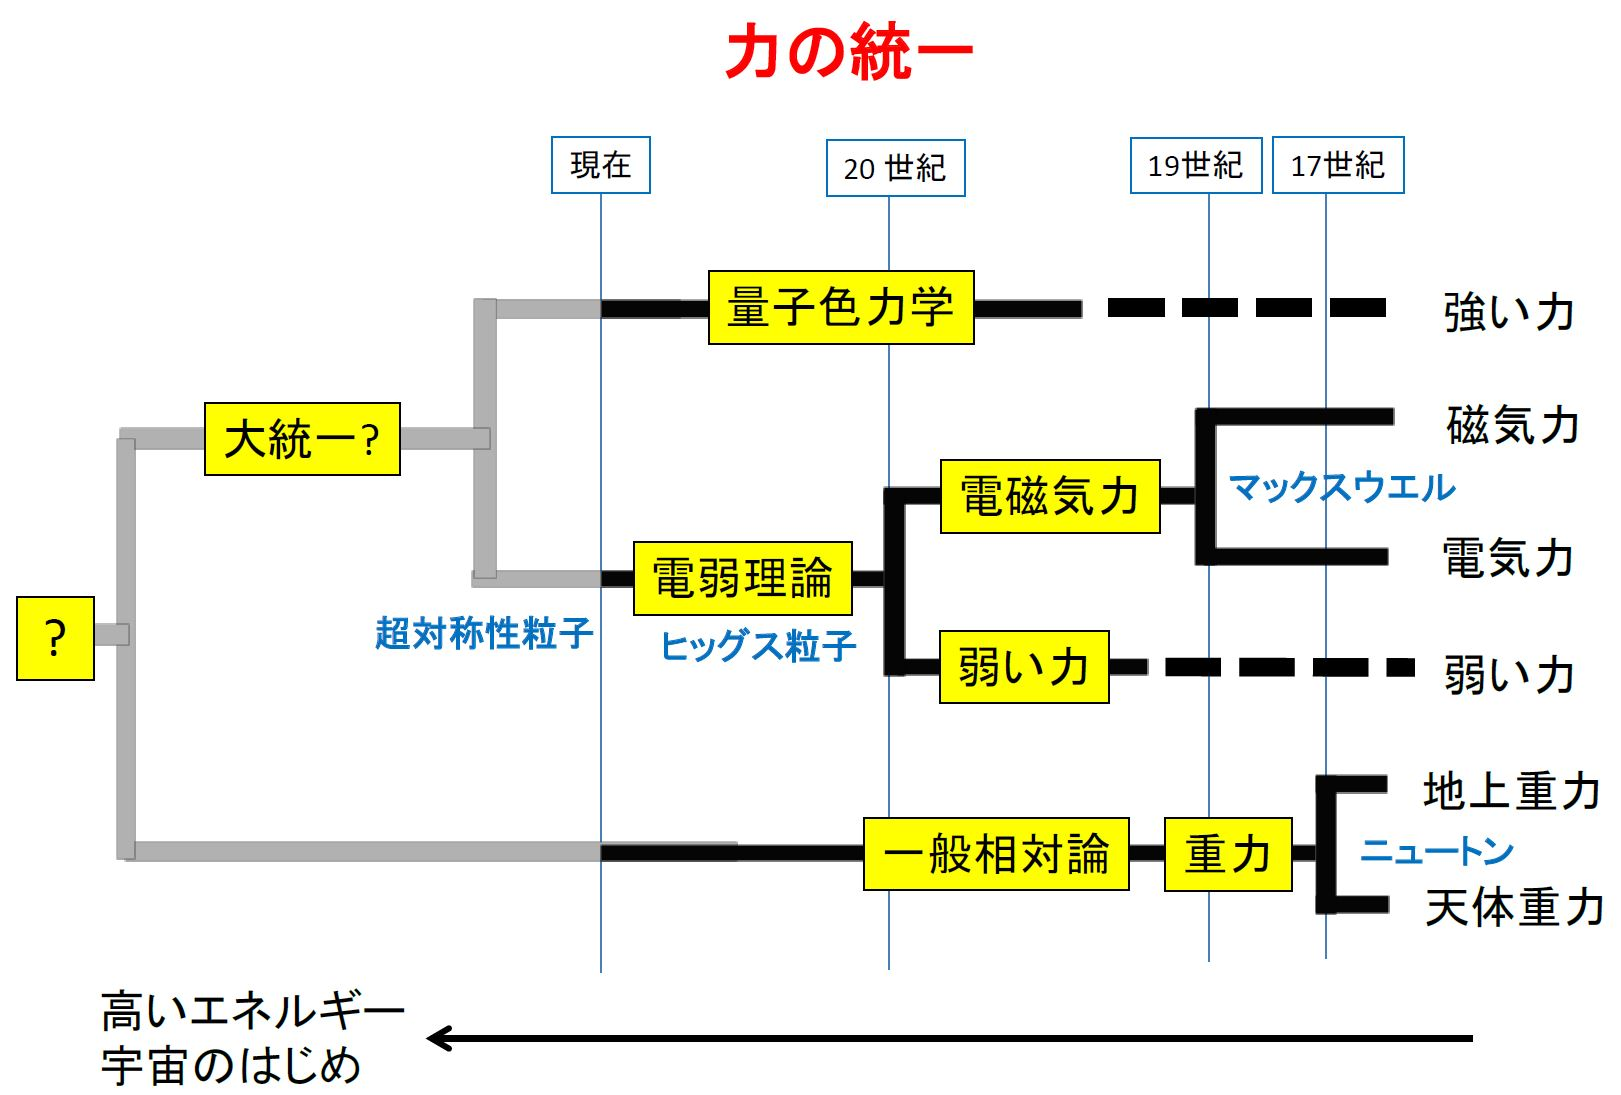
\includegraphics[width=0.9\textwidth]{img/jpeg/physics_bsm_05.jpg}
        \caption[力の統一を表した概念図]{力の統一を表した概念図~\cite{URL:01}。大統一理論は、電磁相互作用、弱い相互作用および強い相互作用を統一する理論である。}\label{fig:gut}
\end{figure}


さらに、標準模型では説明できない事象の一つとして暗黒物質の存在~\cite{AR:11}がある。暗黒物質は銀河の回転速度の観測からその存在が予言された。質量分布が球対称であることを仮定すると、中心からの距離$r$の位置での回転速度$v$は、\equref{eq:dark}と表現できる。
\begin{align}
    v^2\propto\frac{M(r)}{r} \label{eq:dark}
\end{align}
ここで$M~(r)~$は半径$r$内の全質量を表す。もし銀河が現在観測可能な物質のみで構成されているとするならば、その速度$v$は距離$r$とともに小さくなることが示唆される。しかし、近年の銀河の回転速度の観測結果により速度が減少していないことが分かっている~\cite{AR:16}。これは我々が未観測な物質、すなわち暗黒物質が存在する証拠である。現在の宇宙観測によれば、宇宙には光を発していない暗黒物質が通常の物質の~5~倍以上ものエネルギーを担って存在していることが判明している。これは宇宙の全エネルギーの約$22\%$である。

このような標準模型では説明できない物理を、標準模型を超えた物理、~Beyond~the~Standard~Model~(BSM)~と呼び、ATLAS~実験をはじめとして世界中で~BSM~の発見を目的に実験が行われている。そして標準模型における諸問題を解決するための有力な理論の一つとされているのが超対称性理論である。

\section{超対称性理論}
超対称性~(Supersymmetry~:~SUSY)~とは、ボソンとフェルミオン間の対称性である~\cite{AR:12}~\cite{AR:13}。この対称性は、\secref{sec:BSM}で述べた~標準模型における問題を説明できる非常に興味深い理論である。最小超対称標準模型~(Minimal~Supersymmetric~Standard~Model~:~MSSM)~では、標準模型粒子~(SM~粒子)~のそれぞれに対して、超対称性粒子~(SUSY~粒子、スーパーパートナー)~が存在する~\cite{AR:12}。標準模型ではヒッグス粒子は~1~つであるのに対し、MSSM~ではヒッグス粒子のパートナーであるヒッグシーノは複数存在する。また、光子、$W/Z$ボソンおよびヒッグス粒子のスピン~1/2~のスーパーパートナーは、混合してニュートラリーノ$\Tilde{\chi}^0$とチャージーノ$\Tilde{\chi}^{\pm}$と呼ばれる質量固有状態を与える。グラビティーノは重力を伝えるボソンと考えられている重力子~(グラビトン)~のスーパーパートナーである。\tbref{tb:SUSY}に~SUSY~粒子の一覧を示した。

SM~粒子と~SUSY~粒子には大きく~2~つの違いがある。1~つはスピンである。SM~粒子に対し、SUSY~粒子はスピンが$1/2$ずれただけで、電荷などは等しい。SM~でのフェルミオンに対するスーパーパートナーにはスフェルミオンが対応する。SM~におけるボソンに対してはボシーノが対応する。もう~1~つの違いは質量である。SUSY~粒子は未発見のため、超対称性理論は少なくとも低エネルギー領域では破れていると考えられている。したがって、SUSY~粒子は~SM~粒子より大きいオーダーでの質量を持ち、非常に重いと考えることが一般的である。

超対称性理論では、\equref{eq:Rparity}のように表される$R$-パリティと呼ばれる対称性を仮定している。
\begin{align}
    R = (-1)^{3(B-L)+2S} \label{eq:Rparity}
\end{align}
$S$はスピン、$B$はバリオン数、$L$はレプトン数を示している。
$R$-パリティは、SM~粒子に正、SUSY~粒子に負を付与する対称性である。$R$-パリティが保存する場合、SUSY~粒子は、自身の質量より軽い~SUSY~粒子と~SM~粒子に崩壊する。このとき、最も質量の軽い~SUSY~粒子~(Lightest~SUSY~Particle~:~LSP)~は安定となる。LSP~が~SUSY~粒子におけるどの粒子であるかはモデルによって様々だが、電気的に中性なニュートラリーノやグラビティーノであれば~LSP~は暗黒物質の候補となる。$R$-パリティが保存しない場合、LSP~はより軽い~SM~粒子へと崩壊する。$R$-パリティが破れることを$R$-Parity~Violation~(RPV)~と呼ぶ~\cite{AR:12}。
\figref{fig:GUT}~に示すように、SUSY~を仮定することで\secref{sec:BSM}で述べた大統一理論における~3~つの結合定数は~GUT~スケールで一致する。

\begin{table}[tbp]
	\centering
	\begin{tabular}{c|c|ccc|c|c} \hline
	& &\multicolumn{3}{c|}{世代}& \multirow{2}{*}{スピン} & \multirow{2}{*}{電 荷} \\
	& &第1&第2&第3&  &  \\ \hline
	\multirow{4}{*}{スフェルミオン} & \multirow{2}{*}{スクォーク} & $\Tilde{u}$ & $\Tilde{c}$ & $\Tilde{t}$ & 0 & +2/3 \\
	&  & $\Tilde{d}$ & $\Tilde{s}$ & $\Tilde{b}$ & 0 & -1/3 \\ \cline{2-5}
	& \multirow{2}{*}{スレプトン} & $\Tilde{\nu_e}$ & $\Tilde{\nu_{\mu}}$ & $\Tilde{\nu_{\tau}}$ & 0 & 0 \\
	&  & $\Tilde{e}$ & $\Tilde{\mu}$ & $\Tilde{\tau}$ & 0 & -1 \\ \hline\hline
	\multirow{5}{*}{ボシーノ} & ニュートラリーノ& \multicolumn{3}{c|}{\multirow{2}{*}{$\Tilde{\gamma},~\Tilde{Z}^0,~\Tilde{H}^{0}_1,~\Tilde{H}^{0}_2$}}& \multirow{2}{*}{1/2} & \multirow{2}{*}{0} \\
	&~($\Tilde{\chi}^0$)~&  &  & & & \\ \cline{2-5}
	& チャージーノ& \multicolumn{3}{c|}{\multirow{2}{*}{$\Tilde{W}^{\pm},~\Tilde{H}^{\pm}$}} & \multirow{2}{*}{1/2} & \multirow{2}{*}{$\pm1$} \\
	& ~($\Tilde{\chi}^{\pm}$)~ & &&&& \\ \cline{2-5}
	& グルイーノ & \multicolumn{3}{c|}{$\Tilde{g}$} & 1/2 & 0 \\ \cline{2-5}
	& グラビティーノ & \multicolumn{3}{c|}{$\Tilde{G}$} & 3/2 & 0 \\ \hline
	\end{tabular}
	\caption[超対称性粒子の一覧]{超対称性粒子の一覧~\cite{AR:12}。}
	\label{tb:SUSY}
\end{table}

\begin{figure}[H]
        \centering   
        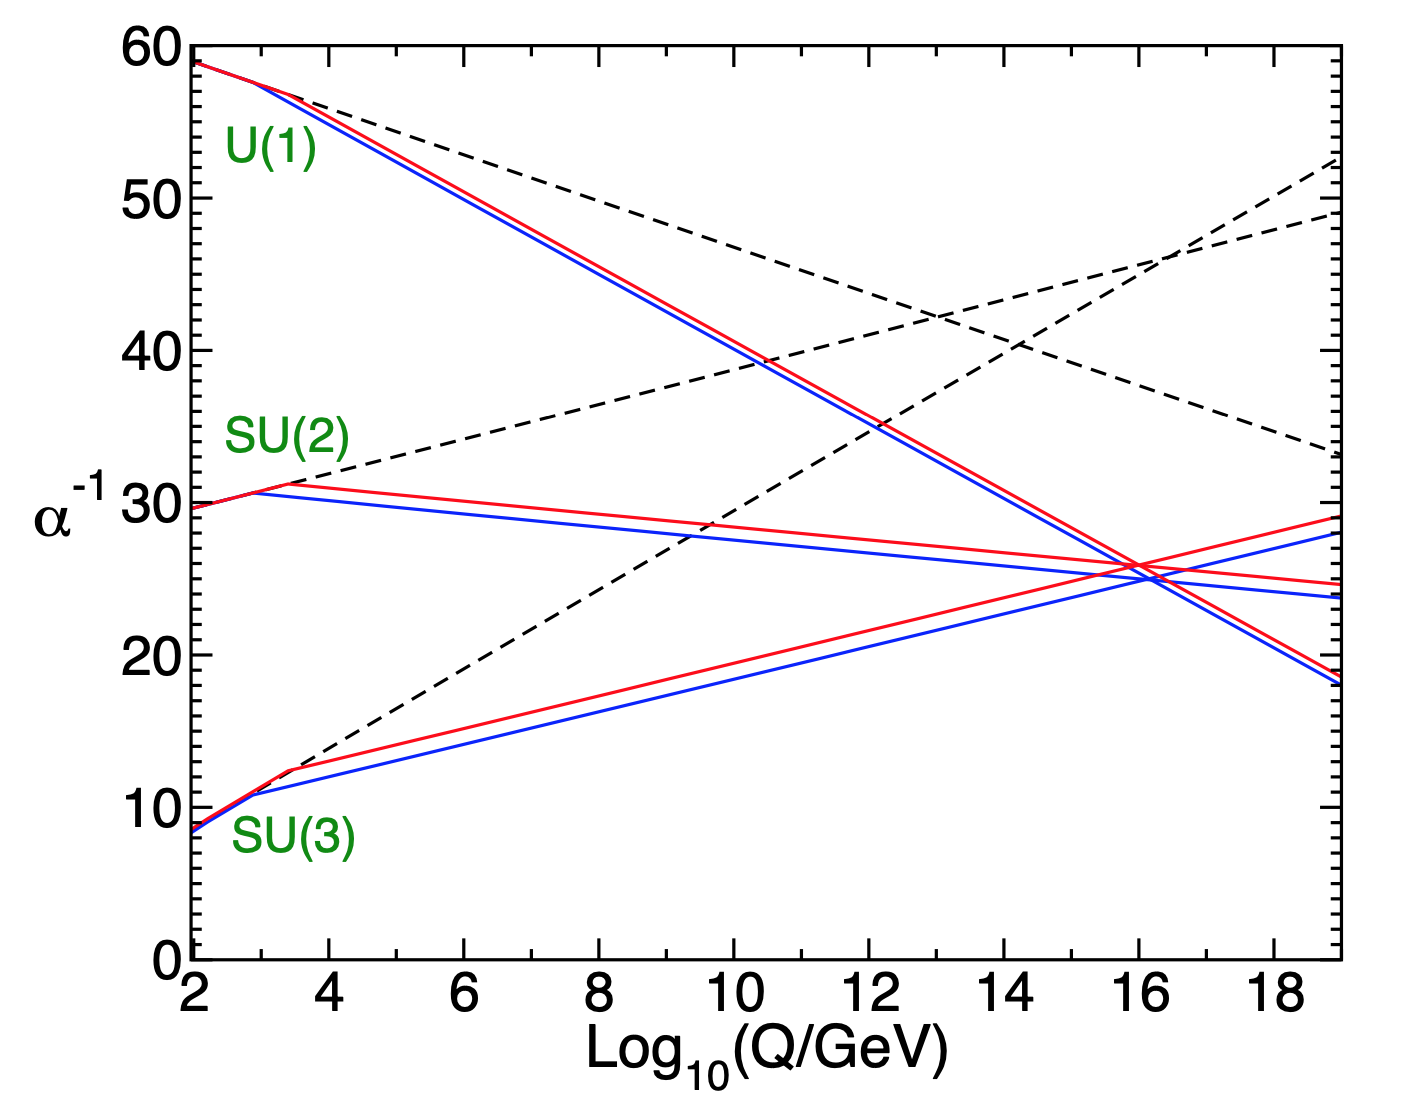
\includegraphics[width=0.85\textwidth]{img/pdf/gut.png}
        \caption[各相互作用における結合定数とエネルギーの関係]{各相互作用における結合定数とエネルギーの関係~\cite{AR:01} 。破線は~SM、実線は~MSSM~を示している。U(1)、SU(2)、SU(3)はゲージ対称性を表し、それぞれ電磁相互作用、弱い相互作用、強い相互作用に対応する。}
        \label{fig:GUT}
\end{figure}

また~SUSY~の枠組みでは$\rm{tan}\beta$という自由パラメータが本質的に重要な働きをする~\cite{URL:24}。SUSY~では~2~種類のヒッグス粒子$\left(H_{\rm{u}}^0,~H_{\rm{d}}^0\right)$が導入され、$\sqrt{v_{\rm{u}}^2~+~v_{\rm{d}}^2}~=~v$を満たしたそれぞれの真空期待値$(v_{\rm{u}},~v_{\rm{d}})$によって電弱対称性が破れる。$v$は標準模型でのヒッグスの真空期待値を表す。この真空期待値の比を\equref{eq:tan}と定義する。
\begin{align}
    \rm{tan}\beta~=~\frac{\it v_{\rm{u}}}{\it v_{\rm{d}}} \label{eq:tan}
\end{align}
SUSY~におけるゲージ結合定数は$\rm{tan}\beta$の関数として記述することができ、SUSY~においては$\rm{tan}\beta$の数値の仮定のもと探索を行う。

\subsubsection{超対称性粒子の探索結果}
超対称性粒子は、ATLAS~実験並びに~CMS~実験において幅広く探索が進められているが、未だ発見には至っていない。しかし、現在までの~SUSY~探索により~SUSY~粒子には大きな制約が課せられ、存在が許される粒子の質量領域が少なくなってきている。\figref{fig:susy1}は、ATLAS~の様々な~SUSY~探索における除外質量制限を示している。グルイーノの生成においては約~2.3~TeV、第一世代および第二世代におけるスクォークにおいては約$\rm{600~GeV\sim1.9~TeV}$、第三世代のスクォークにおいては約$\rm{600~GeV\sim1.2~TeV}$、電弱ゲージーノでは約$\rm{400\sim1100~GeV}$、スレプトンの生成においては約$\rm{700~GeV}$までの質量制限を課している。

\begin{figure}[H]
        \centering   
        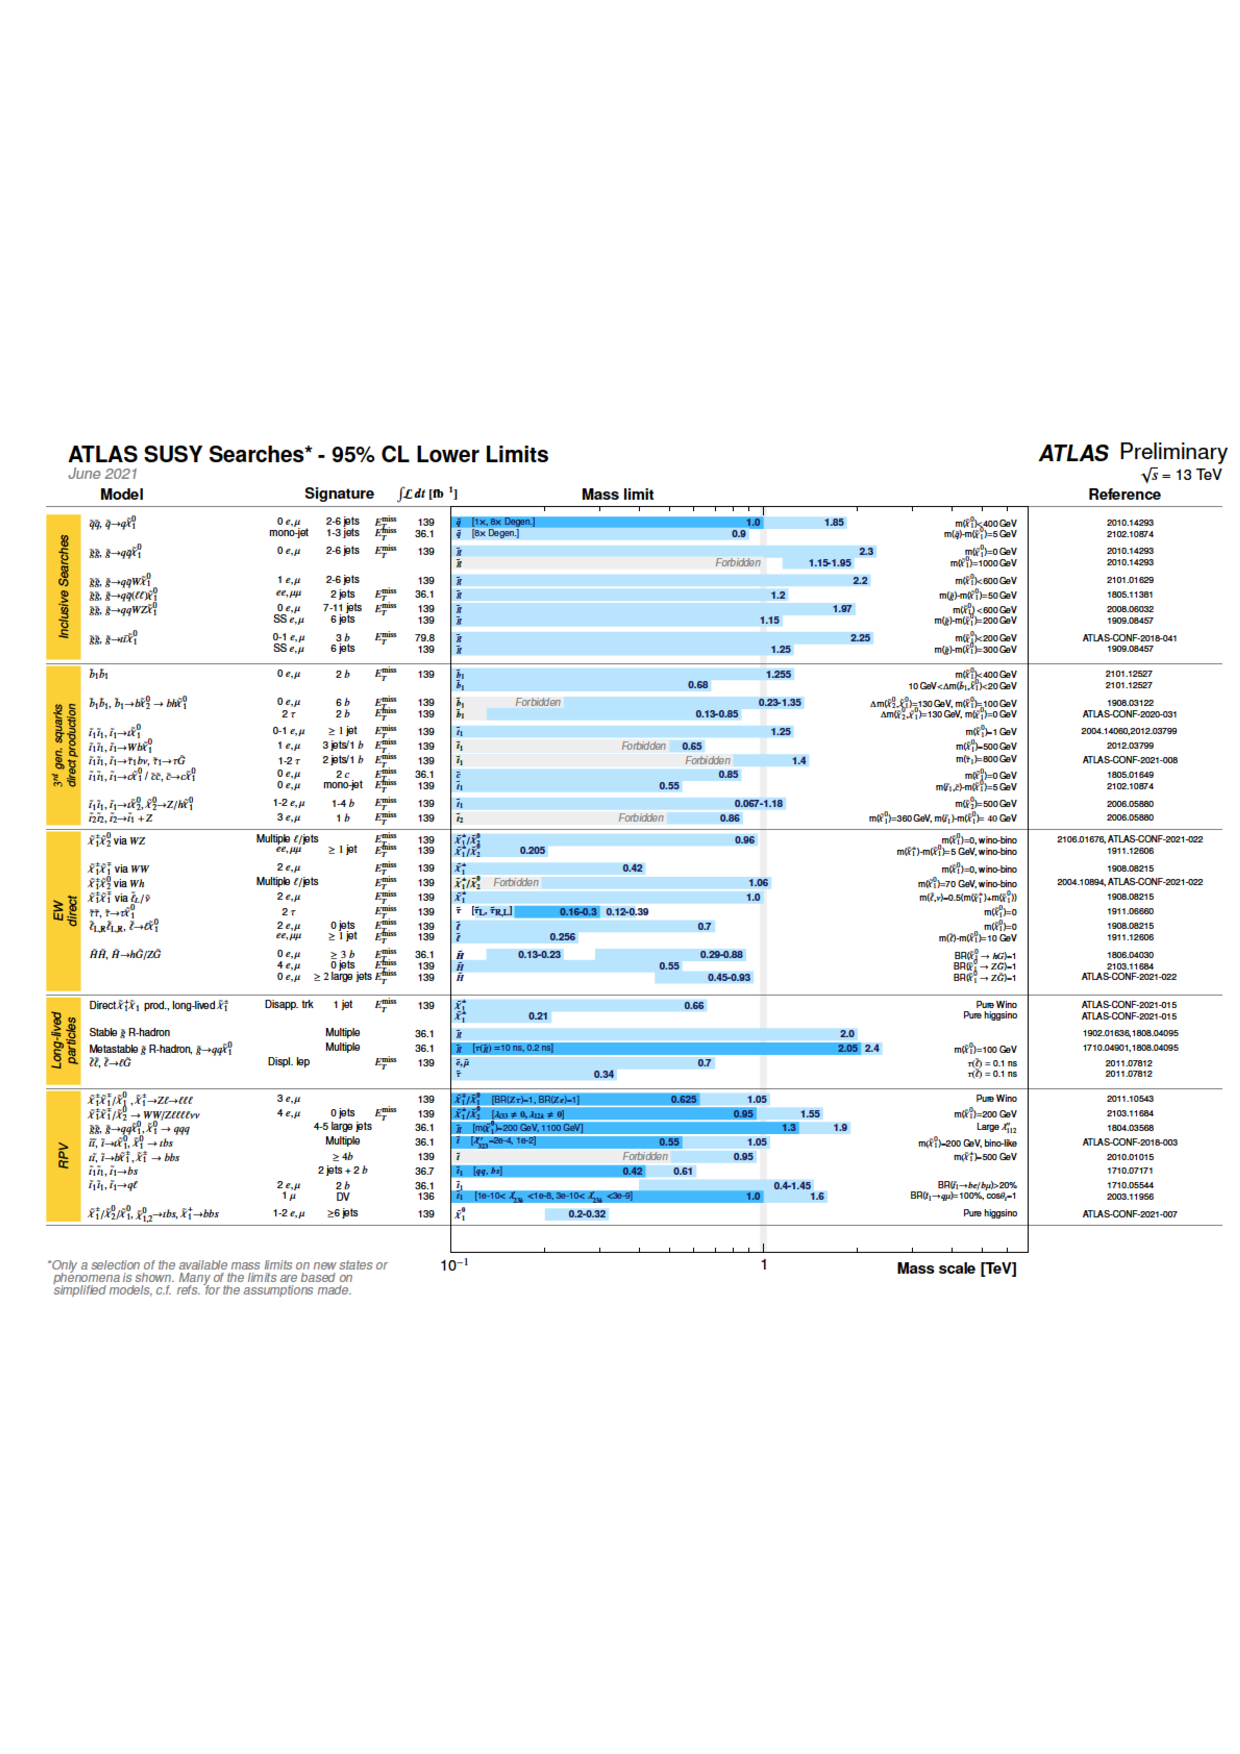
\includegraphics[width=\textwidth,page=1]{img/pdf/susy1.pdf}
        \caption[LHC~での~SUSY~探索の概要]{LHC~での~SUSY~探索の概要~\cite{AR:13}。SUSY~における様々な探索と~ATLAS~の除外質量制限を示している。}\label{fig:susy1}
\end{figure}


\subsection{超対称長寿命粒子}
\label{subsec:LSP}
超対称性のモデルのなかには,崩壊が抑制され長寿命となる粒子を含むものが多数ある。例えば、Gauge~Mediated~Supersymmetry~Breaking~(GMSB)~モデル~\cite{AR:12}では、~SUSY~の破れのスケールを考慮して一番軽い超対称性粒子~(LSP)~はグラビティーノとなる。そしてグラビティーノと~SUSY~場の結合は著しく弱いため二番目の軽い超対称性粒子~(Next~to~Lightest~Supersymmetric~Particle~:~NLSP)~であるスタウ粒子の寿命が長くなると考えられている。

Anomaly~mediation~モデル~\cite{AR:12}では,LSP、~NLSP~がチャージーノになり~質量が縮退し、NLSP~である荷電チャージーノは検出可能な寿命$c\tau~=\mathcal{O}(\rm{1}\sim\rm{10}~\rm{cm})$を持つようになる。

またゲージーノの質量は約~1~TeV~であるが、split~SUSY~モデル~\cite{AR:12}ではスカラー粒子の質量が~1~TeV~より重くなると~生成されたグルイーノの寿命が長くなり、グルイーノが標準モデルクォークと結合して無色化した$R$-ハドロンとよばれる状態になる。\figref{fig:dia}に~GMSB,~Anomaly~mediation,~split~SUSY~の各モデルにおいて予測されている粒子崩壊課程の一例を示した。

\begin{figure}[H]
	\begin{minipage}{0.49\hsize}
	\centering
    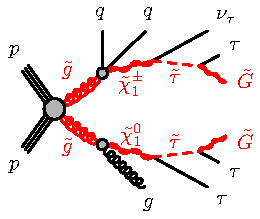
\includegraphics[width=0.7\textwidth]{img/diagram/gogo-qqgtautautauvGG-GMSB.pdf}
    \subcaption{}
    \end{minipage}
    \begin{minipage}{0.49\hsize}
    \centering
    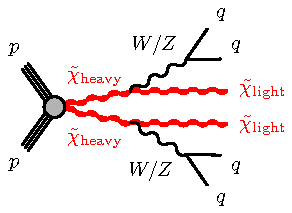
\includegraphics[width=0.7\textwidth]{img/diagram/chichi-qqqq-XX.pdf}
    \subcaption{}
    \end{minipage}\\
    \begin{minipage}{0.98\hsize}
    \centering
    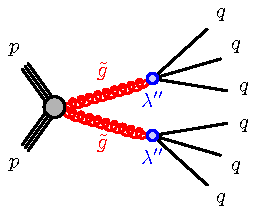
\includegraphics[width=0.35\textwidth]{img/diagram/gogo-3q3q-RPV.pdf}
    \subcaption{}
    \end{minipage}
    \caption[超対称長寿命粒子モデルにおけるファインマンダイアグラムの一例]{超対称長寿命粒子モデルにおけるファインマンダイアグラムの一例~\cite{URL:03}。(a) GMSB モデル。 (b) Anomaly mediation モデル。 (c) split SUSY モデル。}
    \label{fig:dia}
\end{figure}


\subsubsection{重い長寿命粒子の探索結果}
SUSY~における重い長寿命粒子の探索について説明する。\figref{fig:susy2}に~SUSY~における重い長寿命粒子の探索結果を示す。\subsecref{subsec:LSP}で述べた~SUSY~粒子の各モデルにおける様々な探索が行われている。
\begin{figure}[H]
        \centering   
        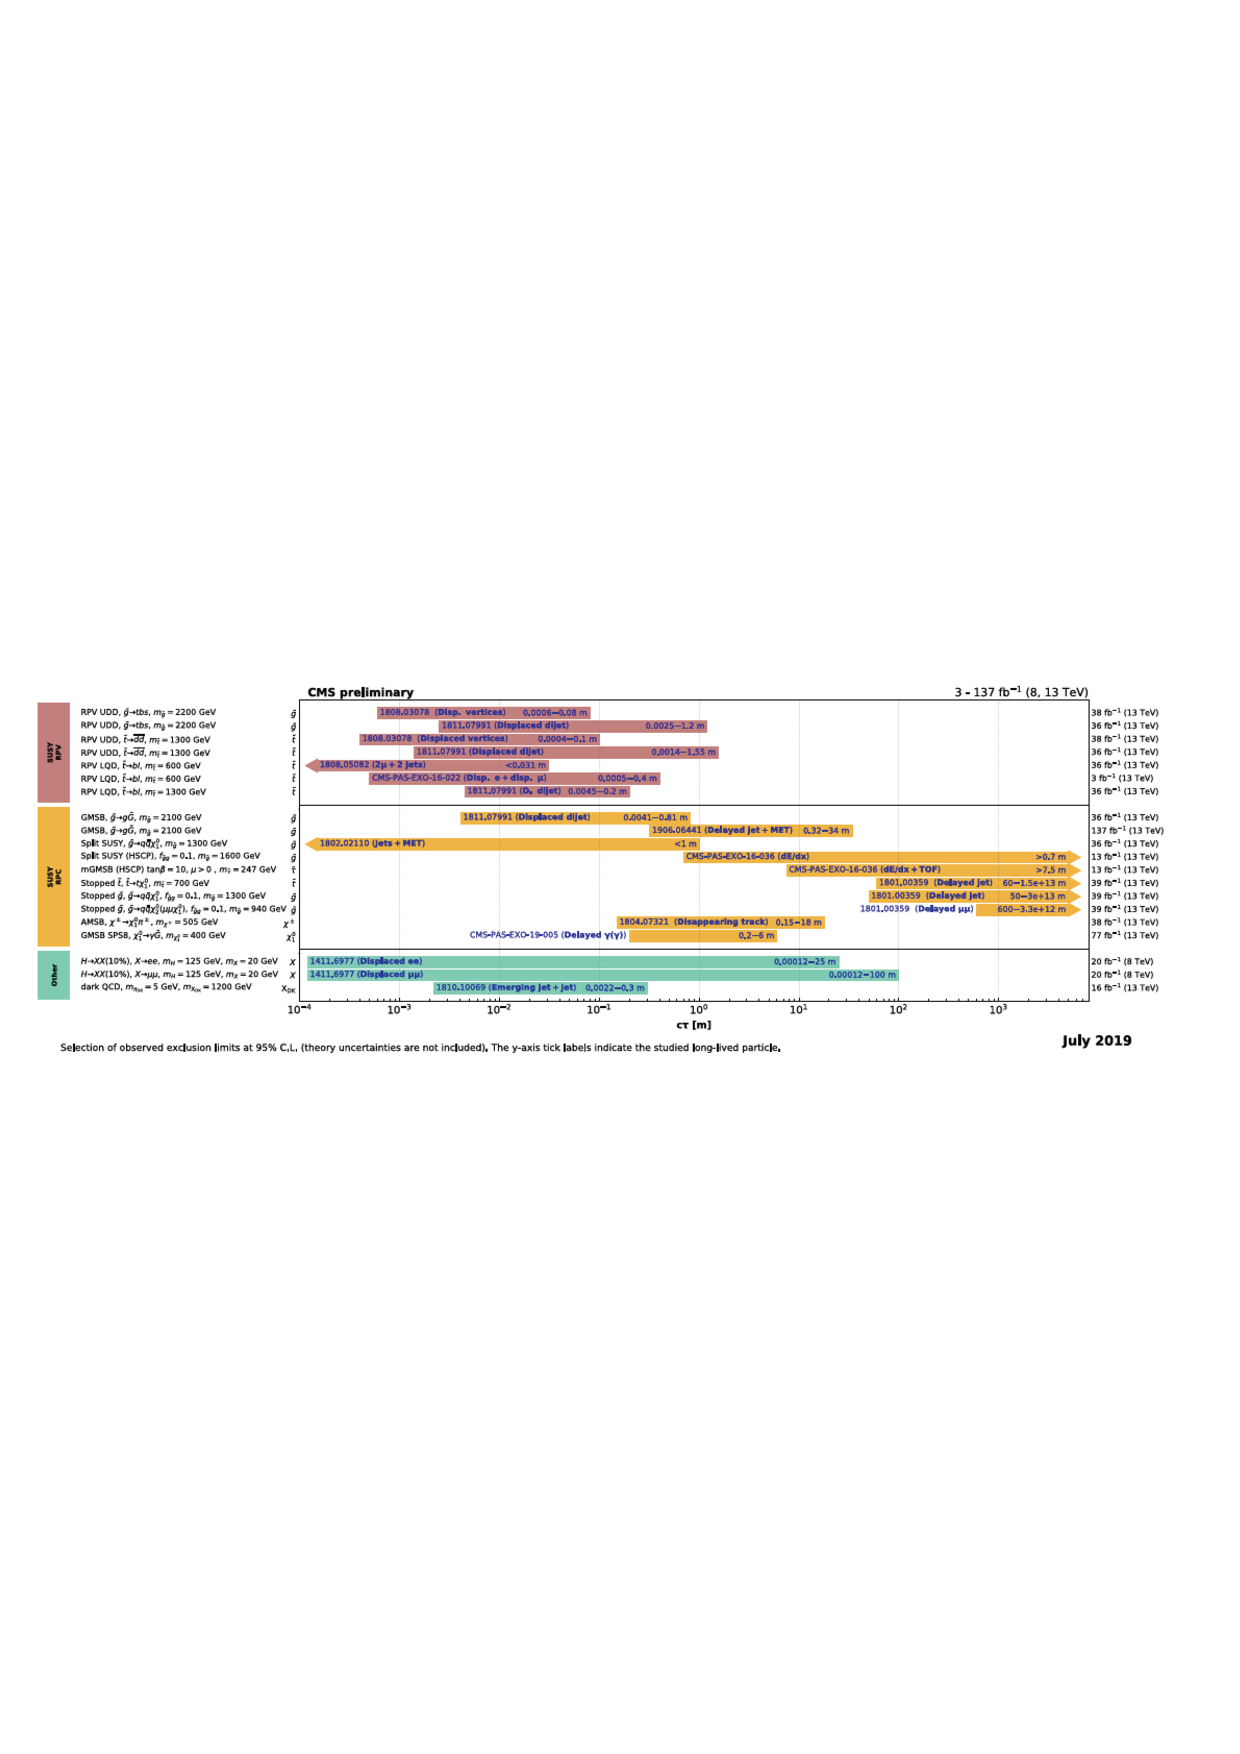
\includegraphics[width=\textwidth,page=1]{img/pdf/susy2.pdf}
        \caption[重い長寿命粒子の探索結果]{重い長寿命粒子の探索結果~\cite{AR:13}。CMS~によって得られた様々な~SUSY~モデルにおける長寿命粒子の$95\%$信頼区間除外領域。横軸は固有崩壊長~($c\tau$)~。}\label{fig:susy2}
\end{figure}

本論文においては、GMSB~モデルにおいて存在が示唆されている長寿命スタウ粒子の探索結果について紹介する。

ATLAS~実験~Run~1~において収集された重心エネルギー$\sqrt{s}~=~8~\rm{TeV}$での陽子陽子衝突による積算ルミノシティ$19.8~\rm{fb}^{-1}$のデータサンプルを使用して、長寿命スタウ粒子の探索が行われた~\cite{AR:03}。推定されたバックグラウンドを超える過剰は観察されず、質量に制限が課せられた。スタウ粒子は、$\rm{10\sim50}$の$\rm{tan}\beta$に対して$\rm{440\sim385~GeV}$の質量まで除外され、スタウ粒子の直接生成のみが考慮される場合は~290~GeV~までの制限を課すことができている。\figref{fig:stau1}に~GMSB~モデルにおけるスタウ粒子の観測結果を示す。

\begin{figure}[H]
    \begin{minipage}{0.49\hsize}
    \centering   
    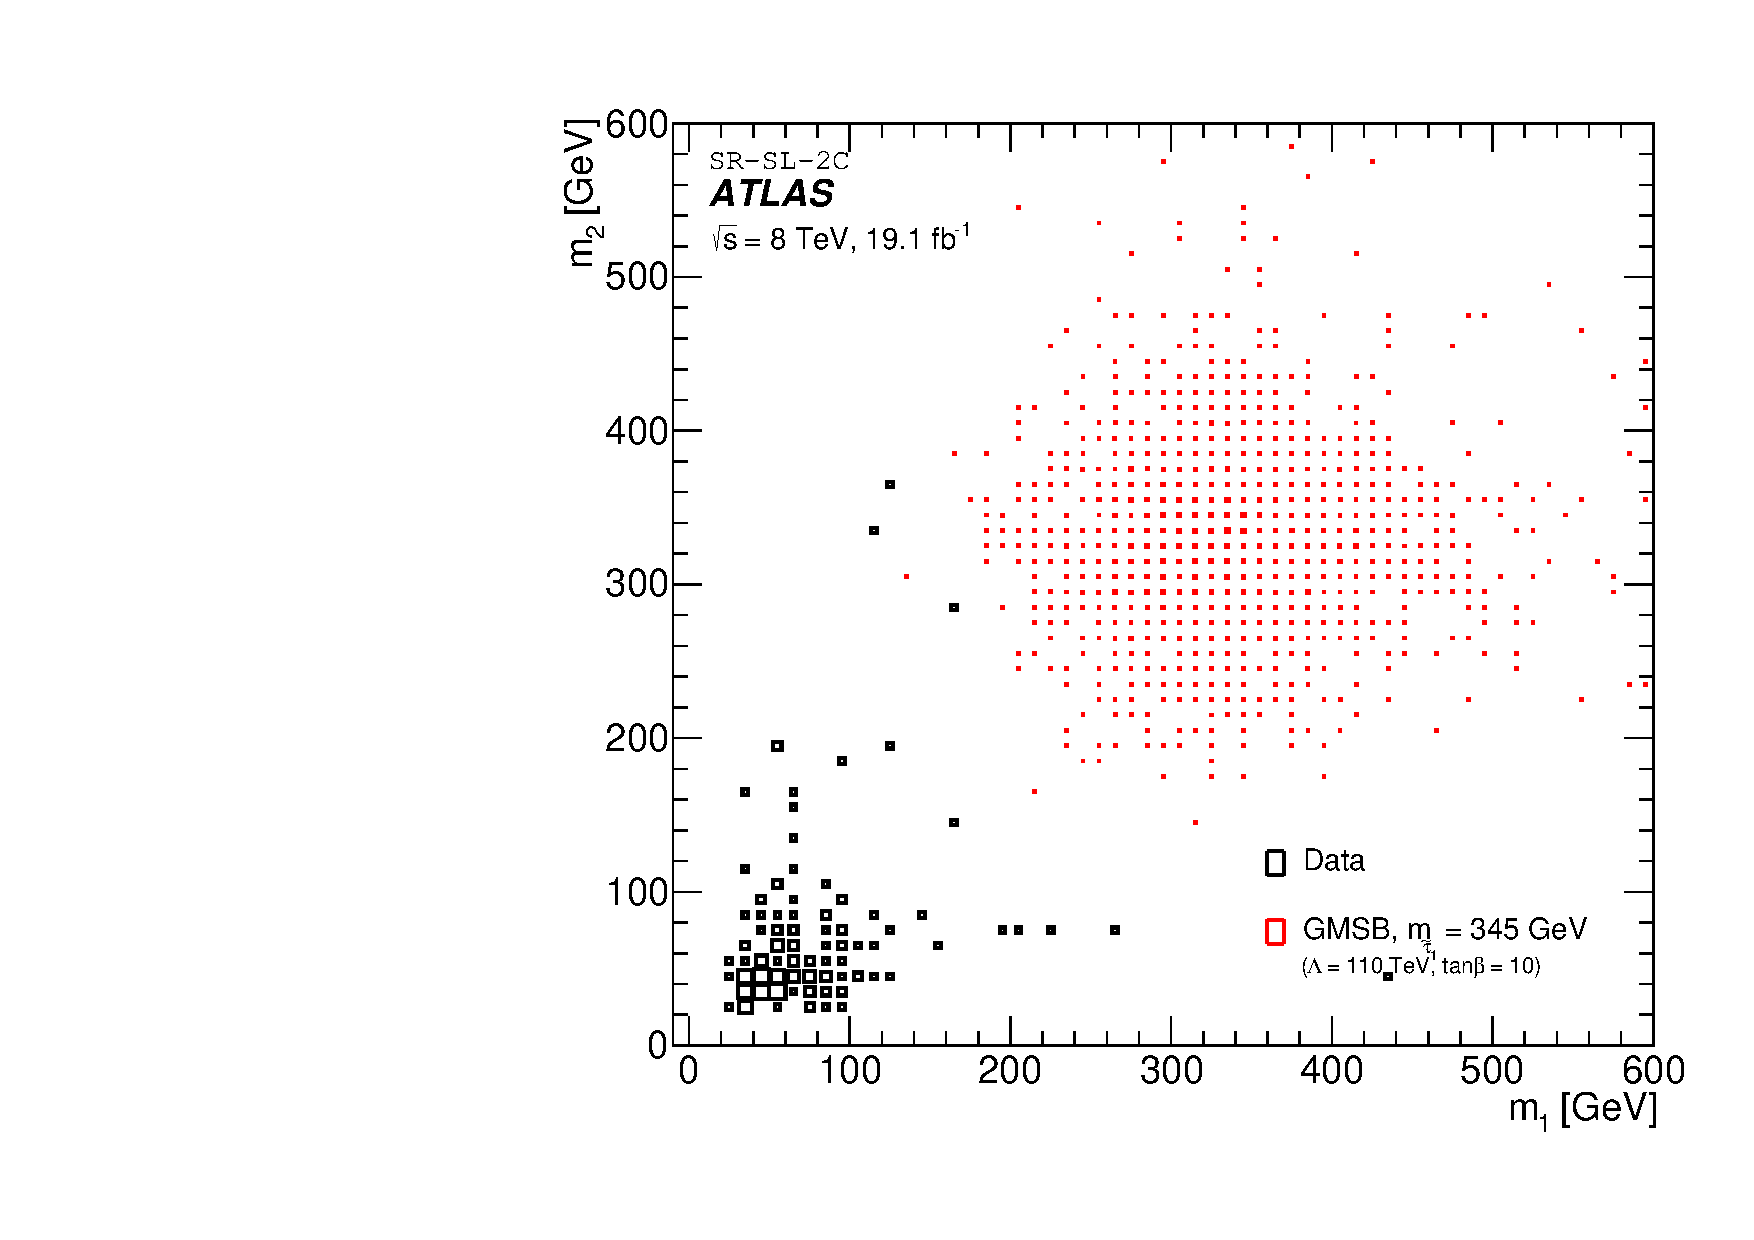
\includegraphics[width=\textwidth]{img/stau/fig_02a.pdf}
    \subcaption{}
    \end{minipage}
    \begin{minipage}{0.49\hsize}
    \centering   
    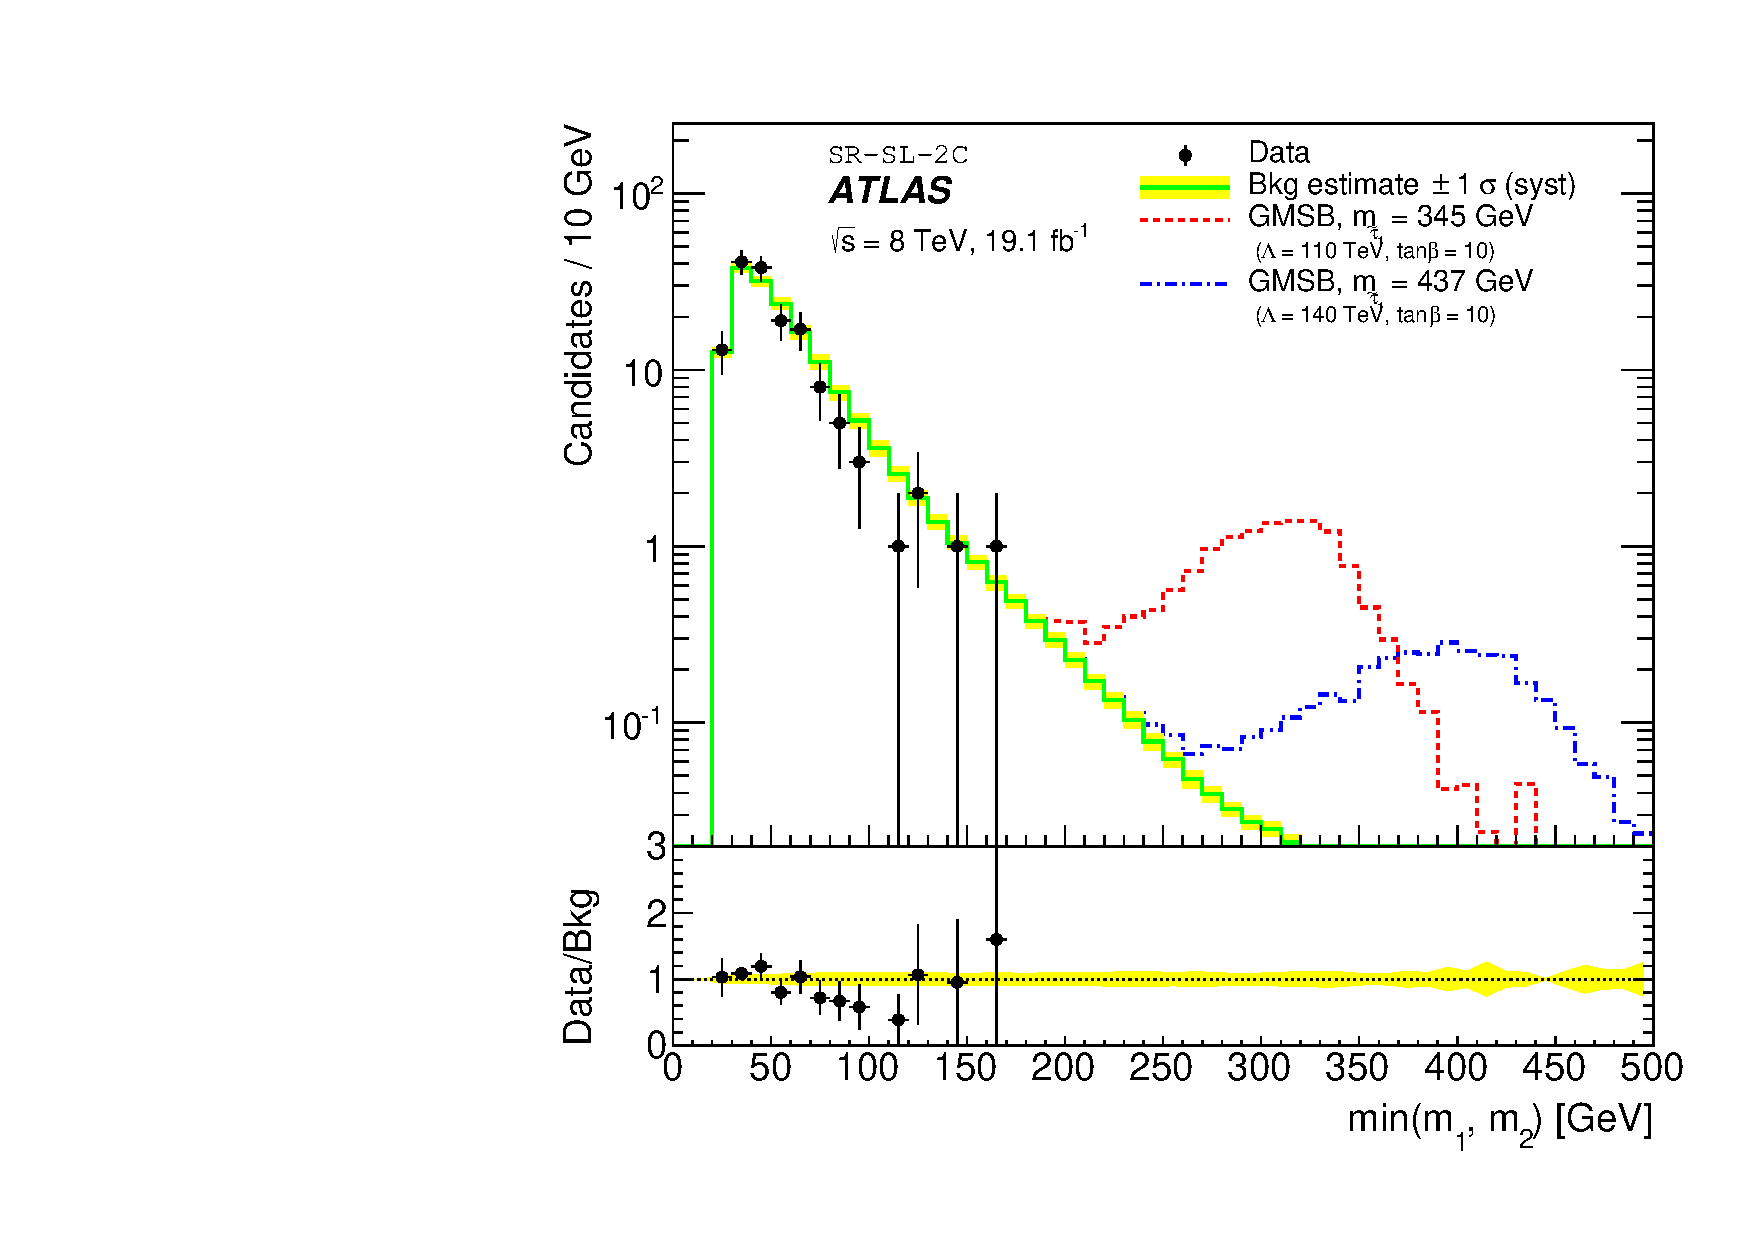
\includegraphics[width=\textwidth]{img/stau/fig_02b.pdf}
    \subcaption{}
    \end{minipage}\\
    \begin{minipage}{0.49\hsize}
    \centering   
    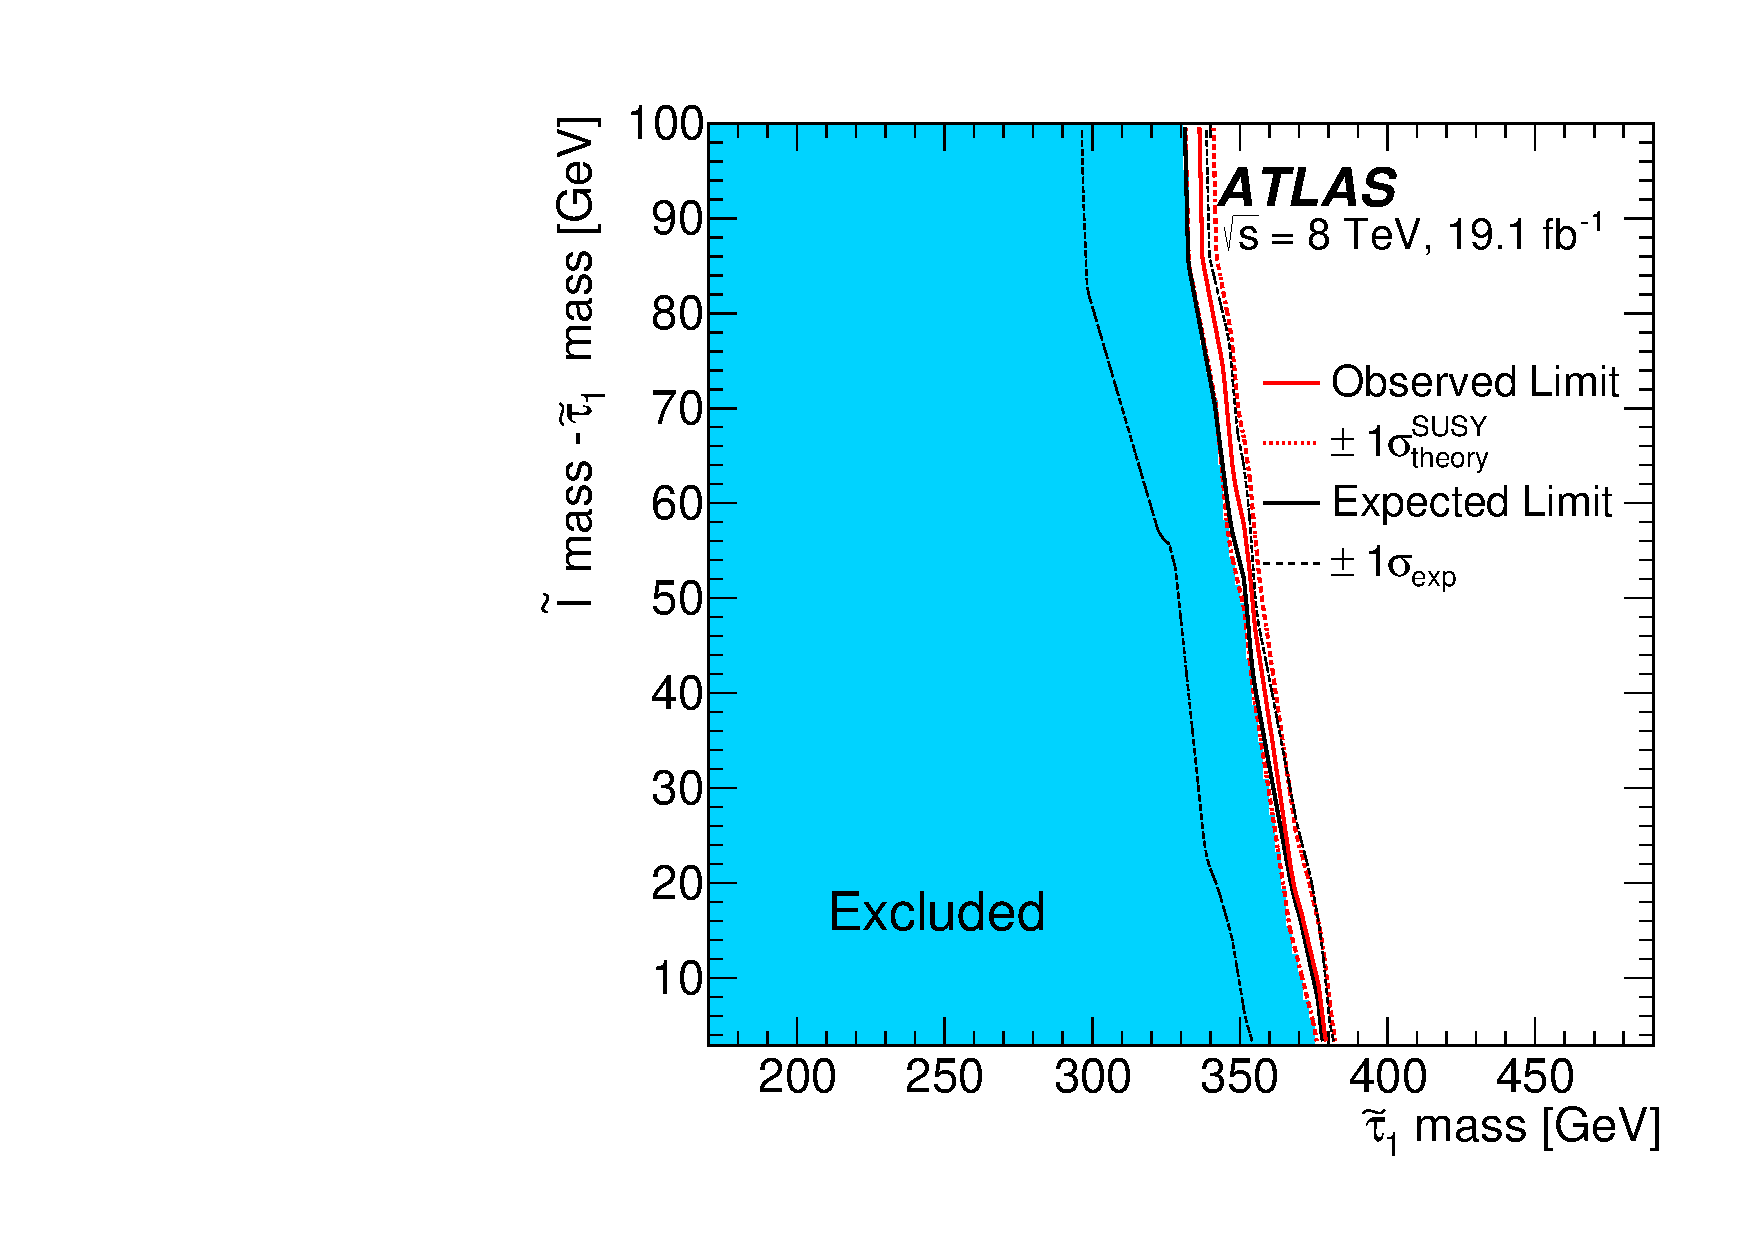
\includegraphics[width=\textwidth]{img/stau/fig_06a.pdf}
    \subcaption{}
    \end{minipage}
    \begin{minipage}{0.49\hsize}
    \centering   
    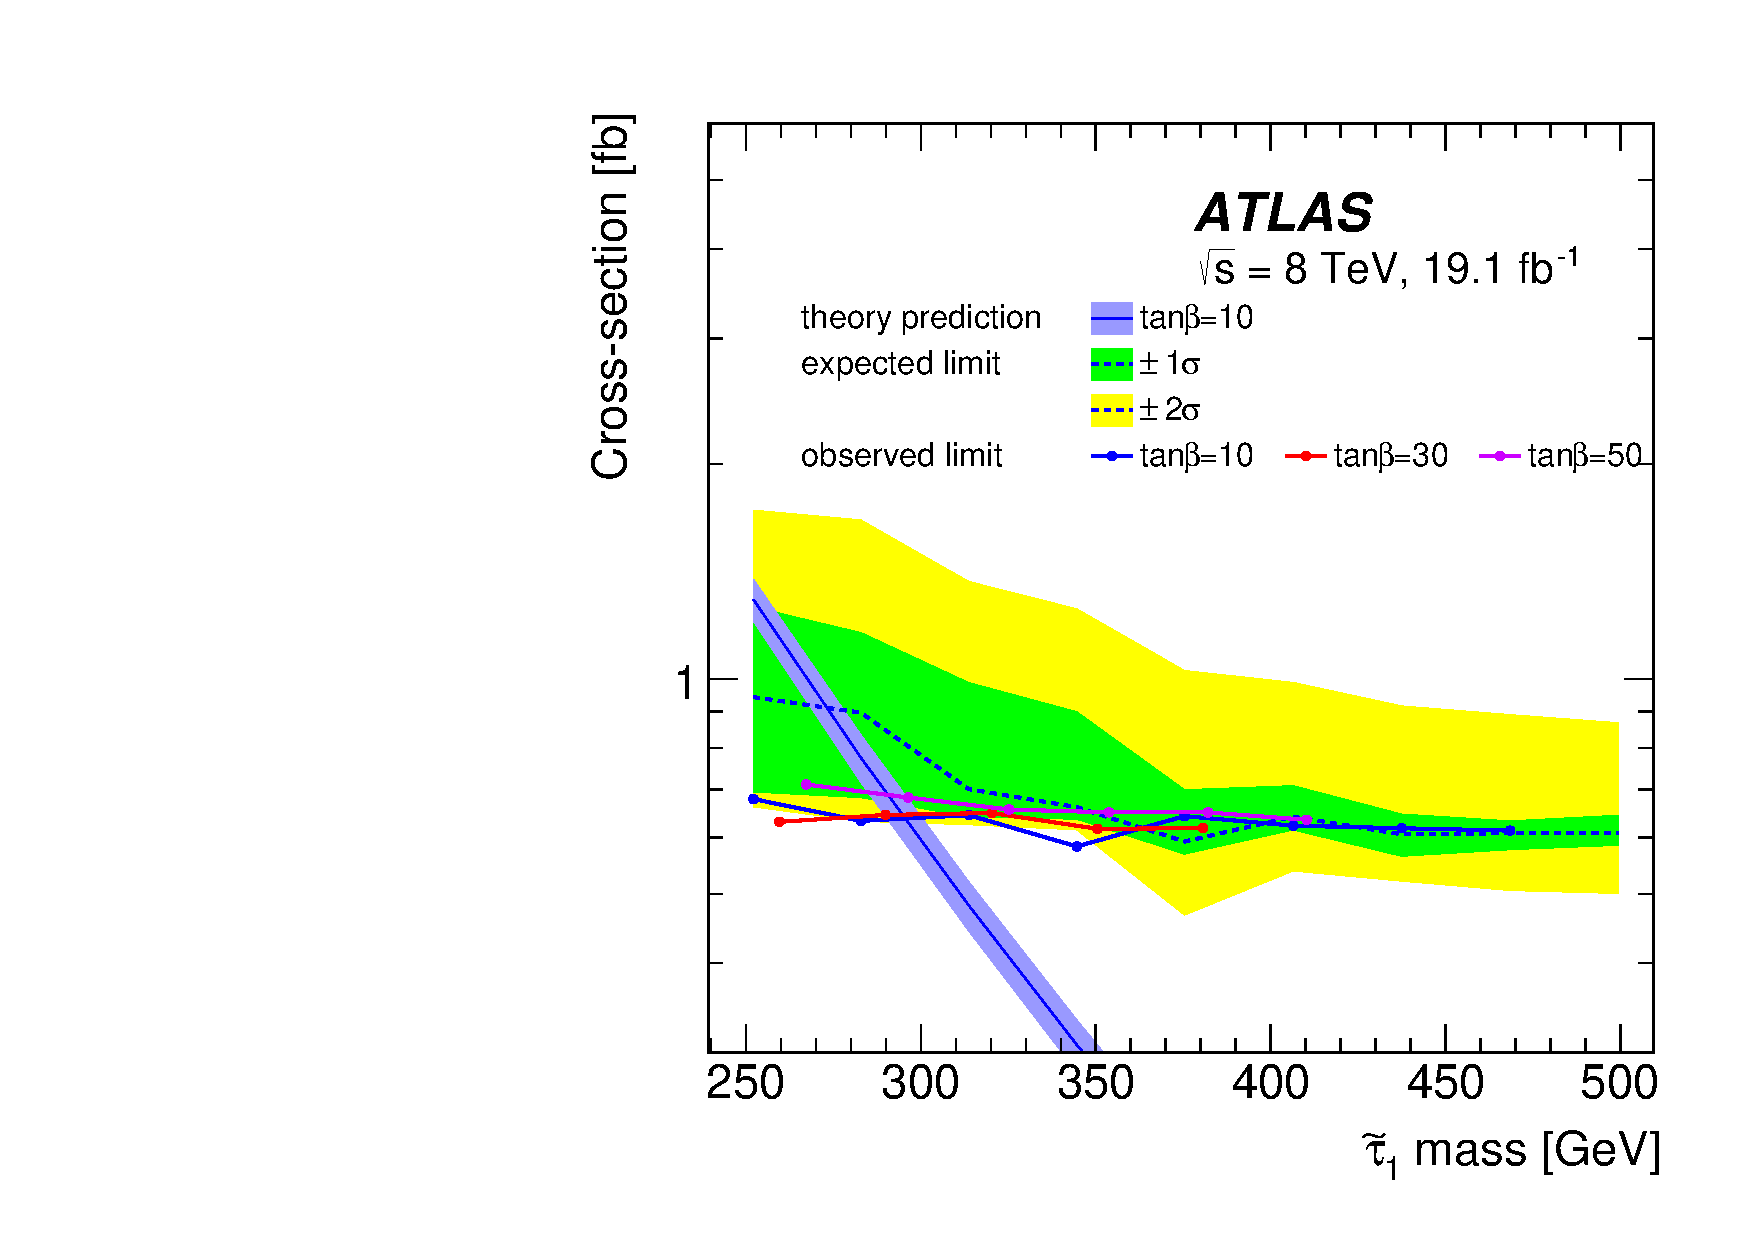
\includegraphics[width=0.99\textwidth]{img/stau/fig_07a.pdf}
    \text{(d)}
    \end{minipage}
    \caption[(a)~GMSB~スレプトン探索における観測データとシミュレーションにおける期待される~1~つの信号候補が再構成された質量$m_{\beta}$の分布。(b)~スレプトンで観測されたデータ、バックグラウンド推定値、および予想される信号。(c)~$95\%$信頼水準における直接生成されたスレプトンの除外領域。(d)~スタウ粒子を直接生成するための質量と$\rm{tan}\beta$の~3~つの値の関数としての断面積の上限。]{(a)~GMSB~スレプトン探索における観測データとシミュレーションにおける期待される~1~つの信号候補が再構成された質量$m_{\beta}$の分布~\cite{AR:03}。(b)~スレプトンで観測されたデータ、バックグラウンド推定値、および予想される信号~\cite{AR:03}~($\it{M}_{\tilde{\tau}}=\rm{345}~\rm{GeV},~\it{M}_{\tilde{\tau}}=\rm{437}~\rm{GeV}$の~2~つの候補信号領域)~。
    (c)~$95\%$信頼水準における直接生成されたスレプトンの除外領域~\cite{AR:03}。除外された領域は青色で表示されている。~予想される制限は黒い実線で描かれ、観測された制限は赤い実線で示されている。(d)~スタウ粒子を直接生成するための質量と$\rm{tan}\beta$の~3~つの値の関数としての断面積の上限~\cite{AR:03}。$\rm{tan}\beta=10$において予想される限界は、それぞれ$\pm1\sigma$と$\pm2\sigma$の不確実性バンドが緑と黄色で描かれている。$\rm{tan}\beta$の~3~つの値で観測された限界は、マーカー付きの実線で示されている。$\rm{tan}\beta=10$の理論的な断面積予測は、色付きの$\pm1\sigma$バンドとして示されている。}\label{fig:stau1}
\end{figure}

\section{スタウ粒子サンプル}
本論文では\subsecref{subsec:LSP}で述べた長寿命スタウ粒子の探索に焦点を当てて研究を行う。
スタウ粒子の特性を理解するためにシミュレーションサンプルを用いて各変数で想定される分布を算出した。\figref{fig:staud1}にスタウ粒子サンプルの$p_{\rm{T}},~\eta$方向における分布を示す。ミューオンは~105~MeV、スタウ粒子サンプルは~600~GeV,~1000~GeV~の質量でシミュレートされたサンプルを使用した。また\figref{fig:staud2}は、各サンプルの粒子速度の分布を示している。スタウ粒子サンプルはミューオンに比べ、非常に質量が大きいため粒子速度の遅い領域まで分布が広がっていることが分かる。ミューオンに関しては、ほぼ光速$\left(\beta~=~1\right)$の領域にしか存在していない。

\begin{figure}[H]
    \begin{minipage}{0.49\hsize}
    \centering   
    \includegraphics[width=\textwidth,page=2]{img/plot/beta.pdf}
    \subcaption{}
    \end{minipage}
    \begin{minipage}{0.49\hsize}
    \centering   
    \includegraphics[width=\textwidth,page=3]{img/plot/beta.pdf}
    \subcaption{}
    \end{minipage}
    \caption[スタウサンプルの$p_{\rm{T}},~\eta,$分布]{スタウサンプルの$p_{\rm{T}},~\eta,$分布。質量が~600~GeV,~1000~GeV~のサンプルを使用した。(a)$p_{\rm{T}}$分布。(b)$\eta$分布。}\label{fig:staud1}
\end{figure}

\begin{figure}[H]
    \begin{minipage}{0.49\hsize}
    \centering   
    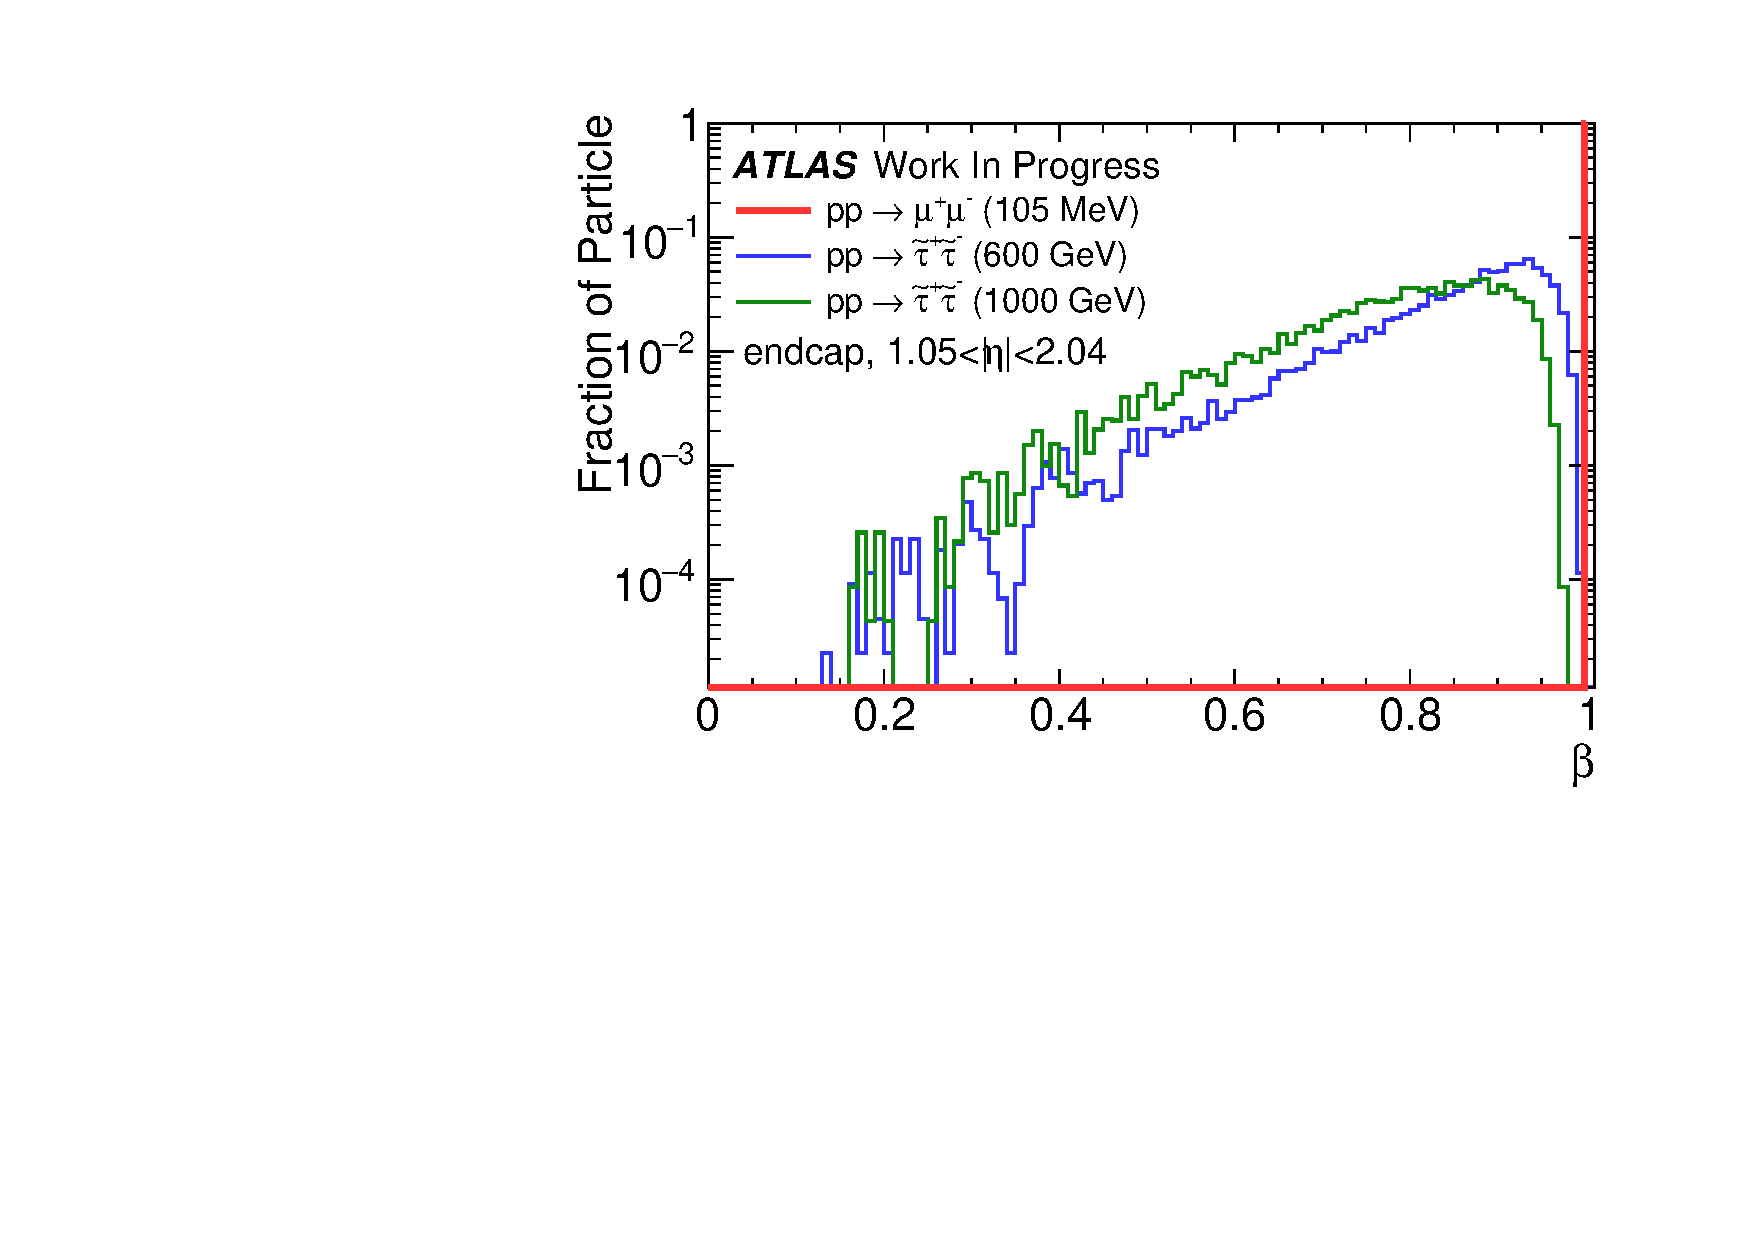
\includegraphics[width=\textwidth,page=1]{img/plot/beta.pdf}
    \subcaption{}
    \end{minipage}
    \begin{minipage}{0.49\hsize}
    \centering   
    \includegraphics[width=\textwidth,page=5]{img/plot/beta.pdf}
    \subcaption{}
    \end{minipage}
    \caption[スタウサンプルとミューオンサンプルにおける粒子速度分布]{スタウサンプルとミューオンサンプルにおける粒子速度分布。ミューオンは質量が~105~MeV,~スタウサンプルは質量が~600~GeV,~1000~GeV~である。(a)~はエンドキャップ領域、(b)~はバレル領域の分布を示す。}\label{fig:staud2}
\end{figure}

\section{シングルミューオントリガー}
\label{sec:single}
本研究で対象としている長寿命スタウ粒子は、寿命が長く安定しているため~ATLAS~検出器の最外に位置するミューオン検出器まで到達すると考えられている。また荷電粒子であるためミューオン検出器での直接検出が可能である。そのため~ATLAS~実験~Run~2~においては標準的なシングルミューオントリガーが解析に用いられていた。\figref{fig:sumi1}は、シングルミューオントリガーにおけるスタウ粒子の取得効率を示している。この図を見ると、スタウ粒子の質量が増加するに従って取得効率が低下していることが確認できる。
$p_{\rm{T}}$閾値~20~GeV~のトリガーの場合、トリガー効率はエンドキャップ領域で約$85\%$であることが知られている。しかし、スタウ粒子のサンプルにおいては$p_{\rm{T}}$が高いにもかかわらず、質量が増加するとトリガー効率が低下し、911~GeV~では約$50\%$に低下している。

\secref{sec:ttri}で述べたようにミューオントリガーは、大きく分けて~L1~と~HLT~の~2~つに分かれている。本節では、それぞれのトリガーの速度の遅い荷電粒子に対する事象選別の特徴と問題点について述べる。

\begin{figure}[H]
        \centering   
        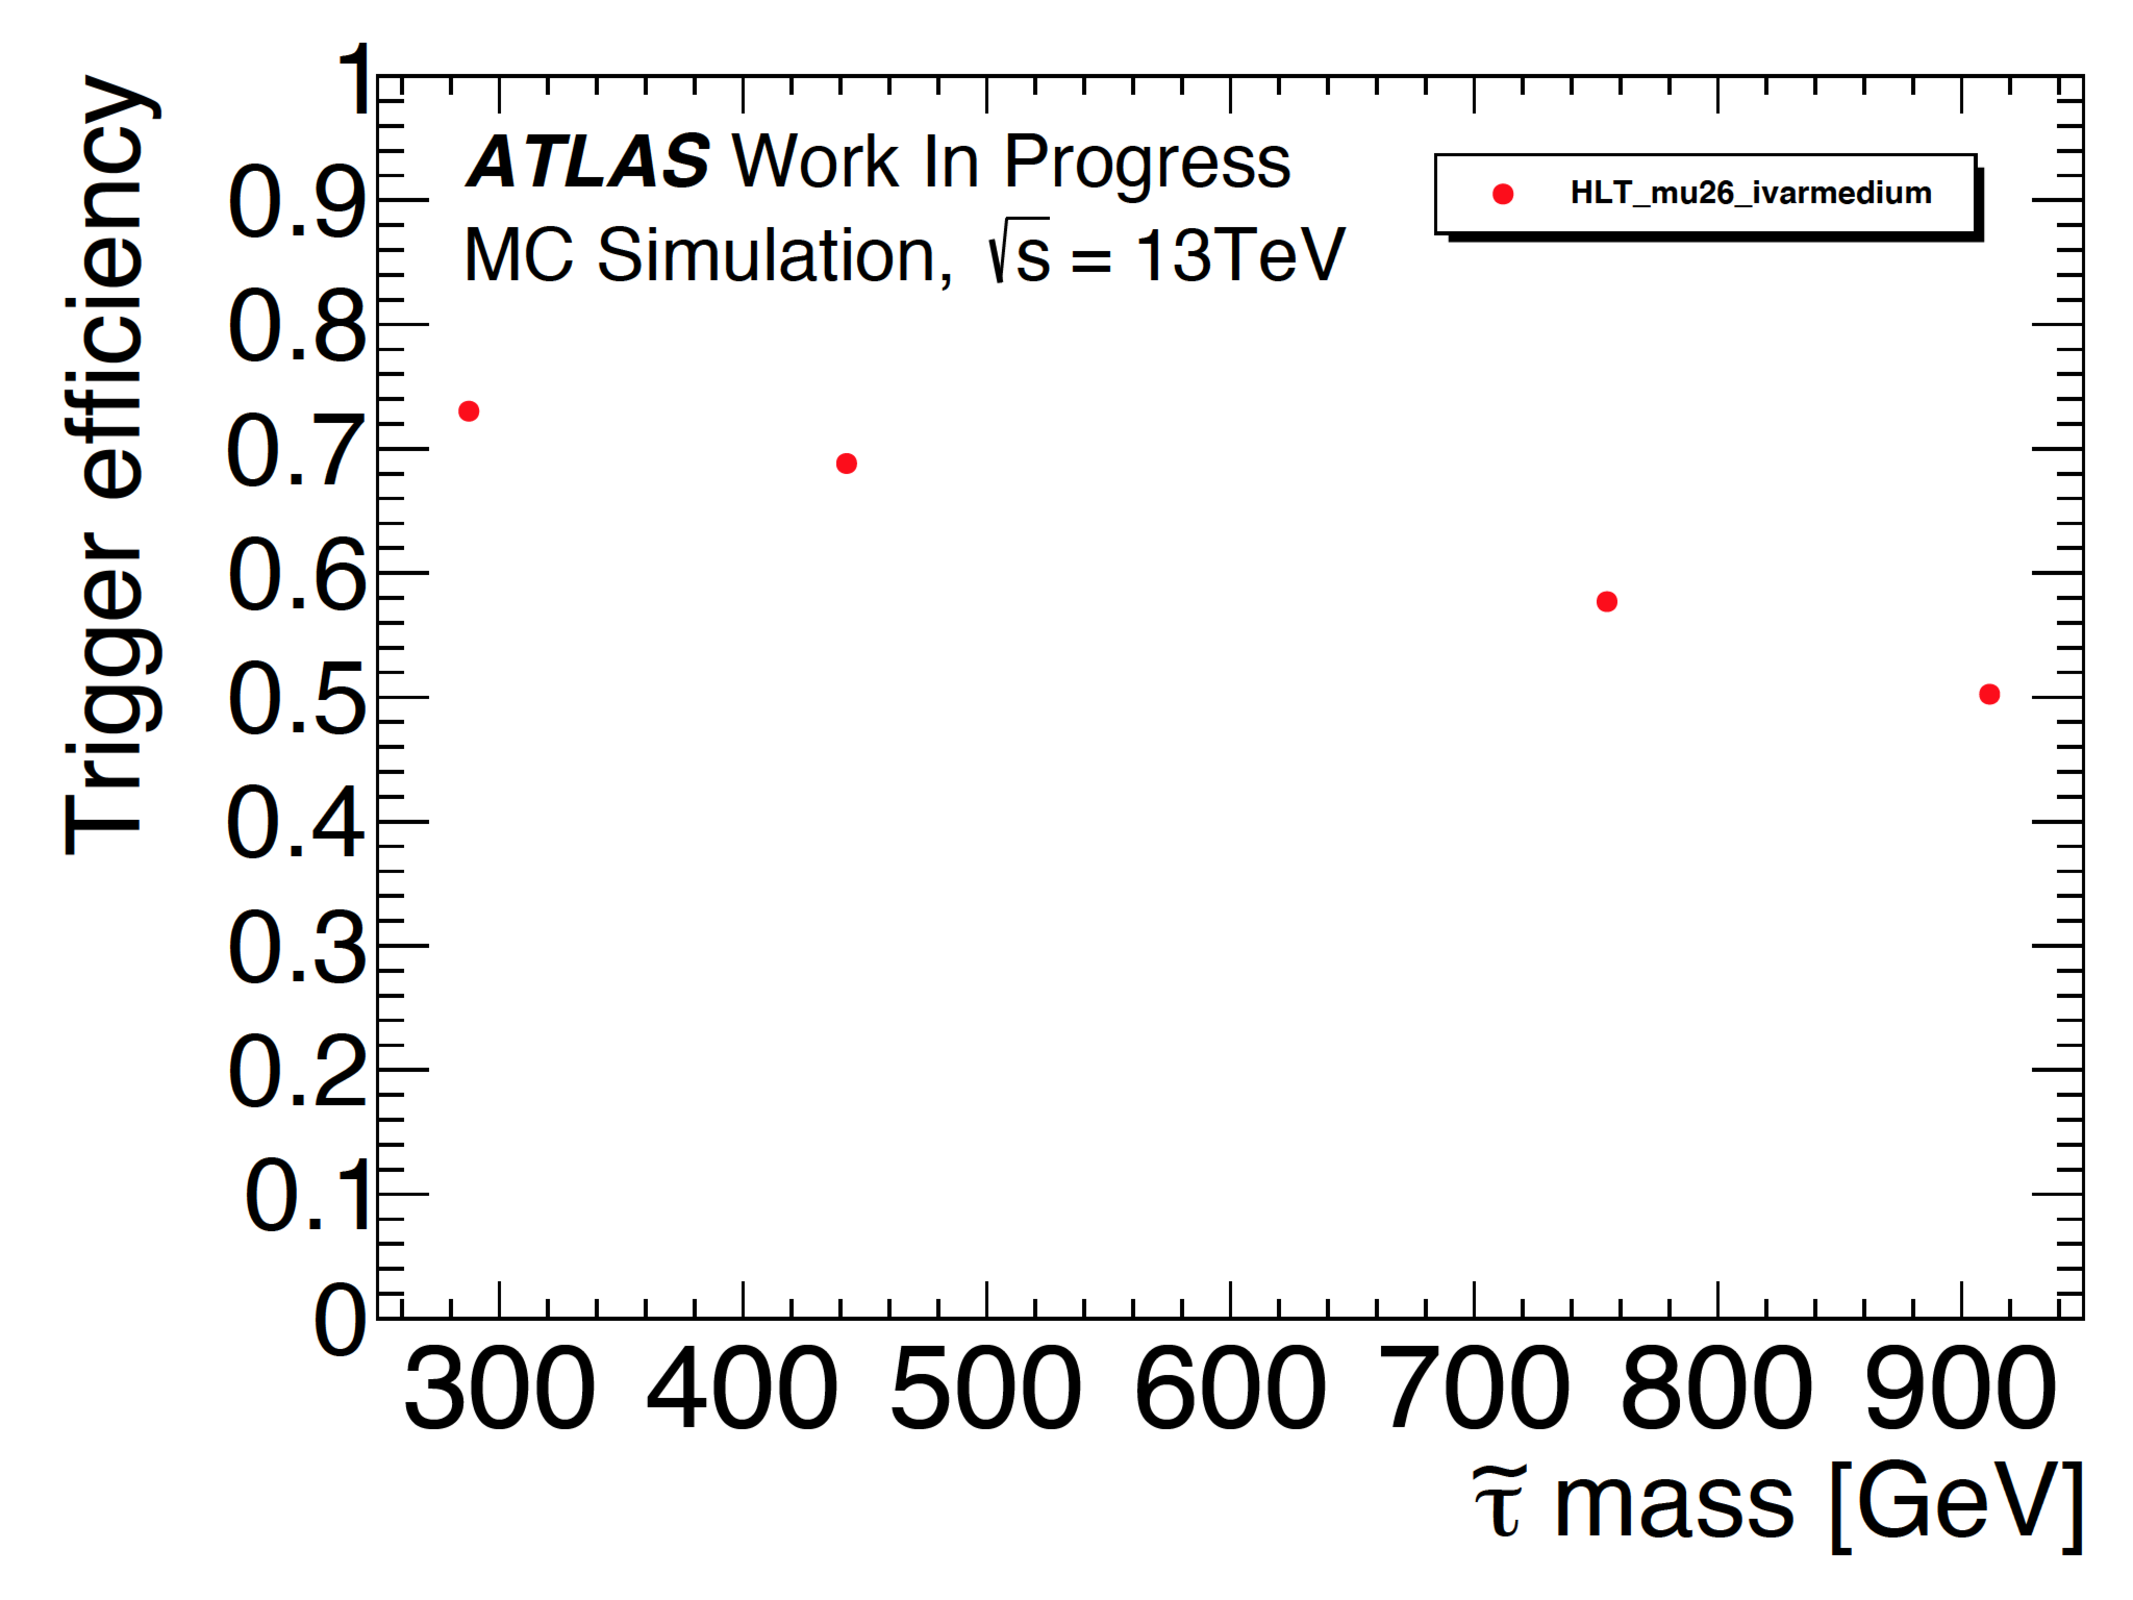
\includegraphics[width=0.7\textwidth,page=1]{img/pdf3/sumi.pdf}
        \caption[シングルミューオントリガーによるスタウ粒子の質量に依存した取得効率]{シングルミューオントリガーによるスタウ粒子の質量に依存した取得効率~\cite{MT:01}。}
        \label{fig:sumi1}
\end{figure}

\subsection{L1~シングルミューオントリガー}
SM~粒子と比べはるかに質量が大きいスタウ粒子では、シングルミューオントリガーにおける取得効率は低下する。これはスタウ粒子の速度が、ほぼ光速の~SM~粒子に比べ、小さいことに由来する。\figref{fig:sumi2}にシングルミューオントリガーによるスタウ粒子の速度に依存した取得効率を示した。標準的なシングルミューオントリガーにおいては$\beta>0.8$の領域にしか感度がないことが分かる。
\secref{sec:ttri}で述べたように~Run~2~のトリガーシステムでは、基本的に粒子が光速で検出器に到達することを仮定している。Run~2~の初期においては、遅い粒子の情報を取得する必要性が認識されておらず、光速の粒子のトリガーを行うことに焦点が当てられていた。したがって、速度の遅い粒子を標準的なシングルミューオントリガーのみでとらえるには限界があり、重い長寿命荷電粒子の探索は標準的なシングルミューオントリガーのみでは不十分であると言える。
\begin{figure}[H]
        \centering   
        \includegraphics[width=0.7\textwidth,page=2]{img/pdf3/sumi.pdf}
        \caption[シングルミューオントリガーによるスタウ粒子の速度に依存した取得効率]{シングルミューオントリガーによるスタウ粒子の速度に依存した取得効率~\cite{MT:01}。}
        \label{fig:sumi2}
\end{figure}

\subsection{HLT~ミューオントリガー}
HLT~ミューオントリガーにおいては、飛跡の再構成のために~MDT~検出器を用いている。MDT~検出器では、荷電粒子が通過することによって電離された電子がセンサーに信号として読みだされるまでのドリフト時間を計算する。
ドリフト速度は一定であるため、ドリフト時間からドリフト半径を求めることができる。実際に荷電粒子が~MDT~検出器を通過する様子を示したものが\figref{fig:mdt}である。複数の~MDT~検出器からドリフト半径を求め、半径の接線を結ぶことにより飛跡の再構成を行う。

粒子の速度が遅い場合、上記の飛跡再構成手法には問題点が存在する。通常のアルゴリズムでは粒子の飛行時間を求める際に、粒子速度が光速であることを仮定して計算が行われている。従って速度の遅い粒子では、飛行時間が長くなるためドリフト半径を誤って本来よりも大きい値として計算してしまう。以上の影響により遅い荷電粒子に対して、誤った飛跡再構成が行われる。
そこで、HLT~の遅い荷電粒子用トリガーにおいては飛行時間が誤っていることを想定し、飛行時間を変化させながら再構成を行うという手法をとる。内部飛跡検出器から外挿された飛跡とのマッチングをとることで飛跡を一意に決定する。
\figref{fig:hlt}に~HLT~におけるトリガー効率を示した。トリガー効率には粒子速度による依存性は見られず、約$80\%$のトリガー効率を達成している。しかし、光速のミューオンに対する~HLT~のトリガー効率は約$90\%$であることが知られている。これは一部の領域においてドリフト時間を変化させるフィッティングによって一意に飛跡を決定できないことが原因である。この問題を解消する方法として、あらかじめ数種類のドリフト時間を仮定し、飛跡候補の選択肢を用意しておく手法が提案されたが、処理時間増加の観点から~Run~3~での導入は難しいと考えられている~\cite{MT:01}。

\begin{figure}[H]
        \centering   
        \includegraphics[width=0.65\textwidth,page=2]{img/pdf3/mdt.png}
        \caption[ミューオンが通過した際の飛跡再構成の様子]{ミューオンが通過した際の飛跡再構成の様子~\cite{MT:01}。各~MDT~ヒットに対するドリフト半径を結んだ接線を求めることで飛跡の再構成を行う。}
        \label{fig:mdt}
\end{figure}

\begin{figure}[H]
        \centering   
        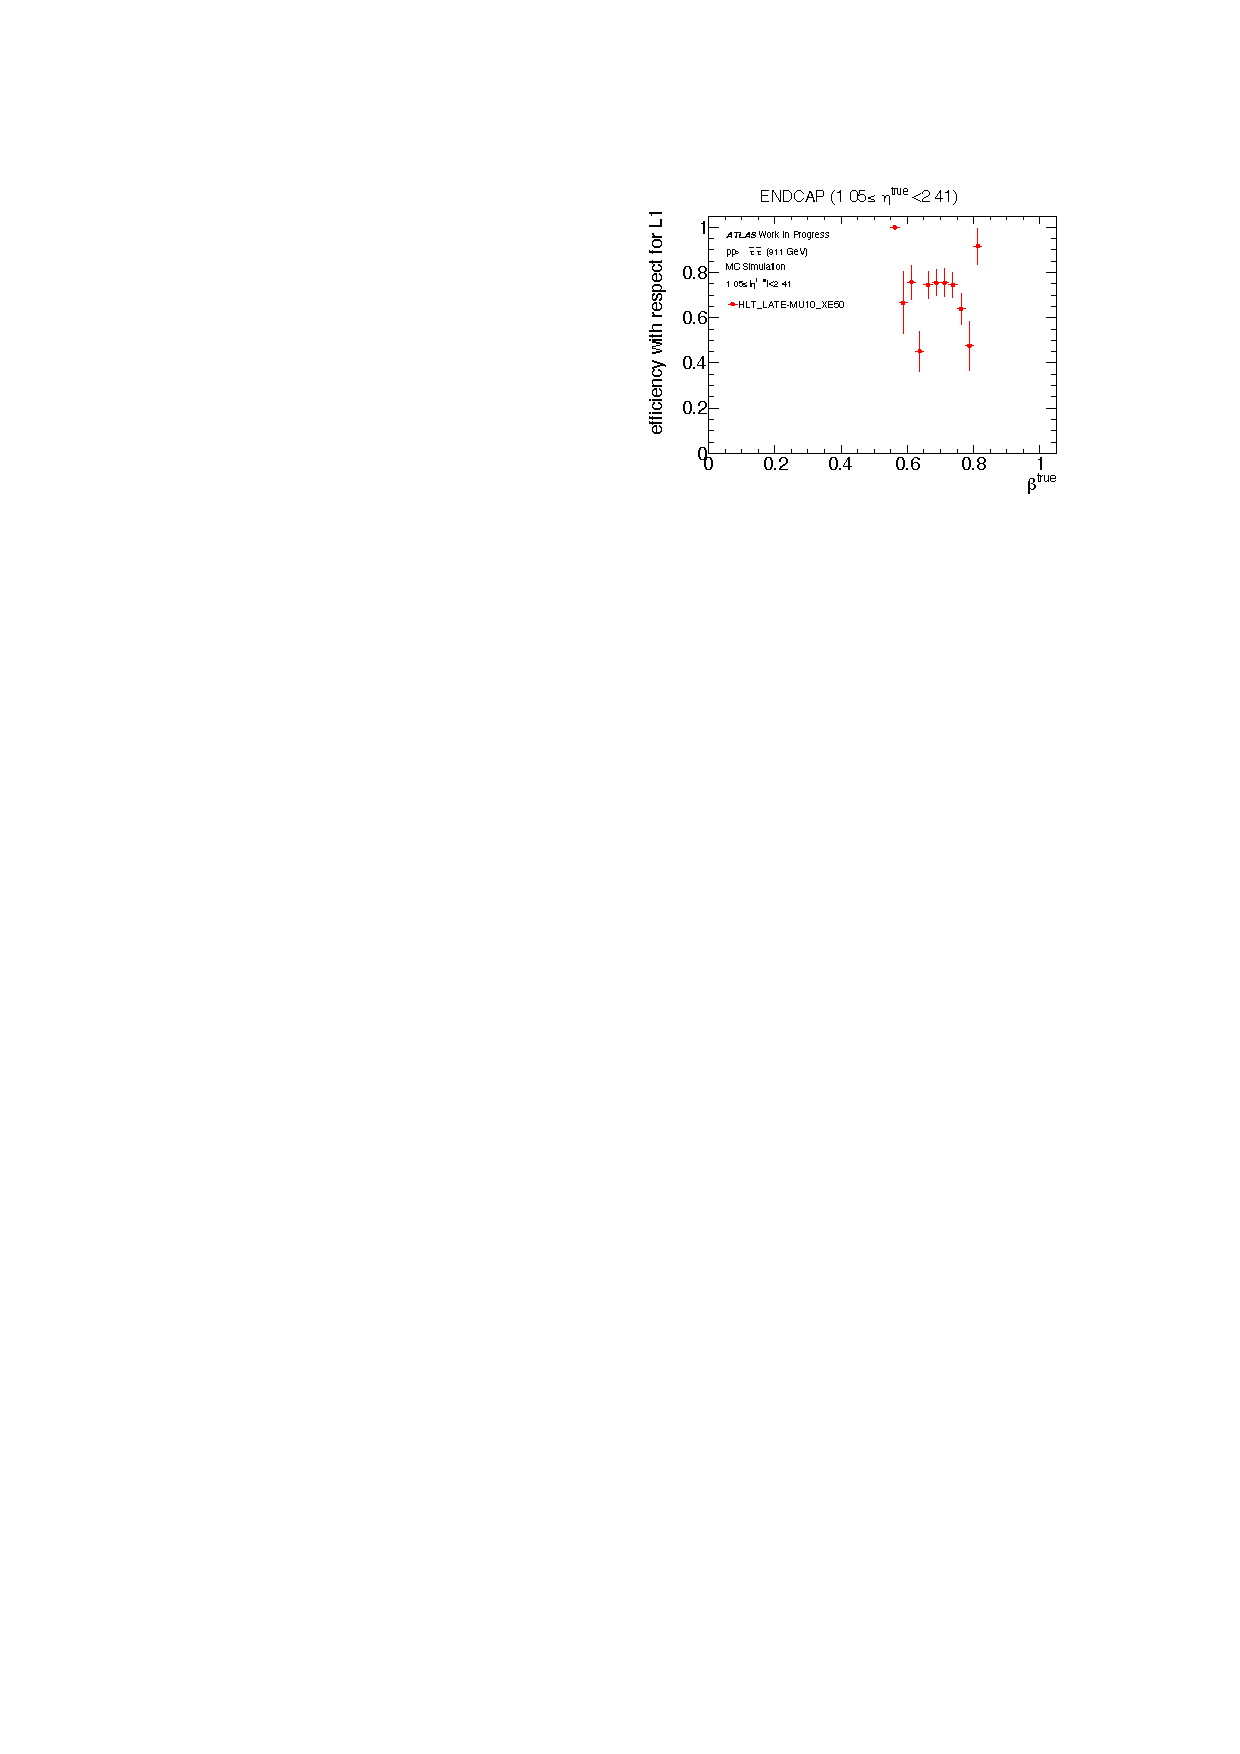
\includegraphics[width=0.75\textwidth,page=1]{img/pdf3/hlt.pdf}
        \caption[エンドキャップ領域における速度に依存した HLT のトリガー効率]{エンドキャップ領域における速度に依存した~HLT~のトリガー効率~\cite{MT:01}。}
        \label{fig:hlt}
\end{figure}

\section{遅い荷電粒子探索用~L1~トリガー}
\label{sec:latemu}
標準的なシングルミューオントリガーでは$\beta{\leq}0.8$の領域にしか感度がなかった。これはL1~シングルミューオントリガーが、基準バンチの情報のみをトリガー判定に利用していたことによるものである。ATLAS~実験においても、速度の遅い荷電粒子探索の必要性が認識され、新たな~L1~の遅い荷電粒子探索用トリガーが~Run~2~の後半に試験的に導入された。このトリガーは速度が遅い粒子の情報を取得するために、基準バンチの次のバンチのタイミングでミューオン検出器に到達した粒子に感度を持つ。しかし、ミューオントリガーのみでトリガー判定を行うと、次バンチであることの保証ができない。実験においては次バンチであることの保証のために、別の検出器で基準バンチのタイミングを要求する。遅い荷電粒子探索用トリガーにおいては、カロリメータで基準バンチに~MET~またはジェットが存在することを要求することでタイミングの保証をしている。\figref{fig:met}に要求する事象のイメージ図を示す。

\figref{fig:sumi3}は、スタウ粒子のシングルミューオントリガー、遅い荷電粒子探索用トリガーおよび~MET~トリガーの速度に依存した取得効率を示している。
遅い荷電粒子探索用トリガーは$0.6{\leq}\beta{\leq}0.8$の領域に感度があることが分かる。トリガー効率が約$30\%$であるのは~MET~トリガーの効率が$30\%$程であることによる。

\begin{figure}[H]
        \centering   
        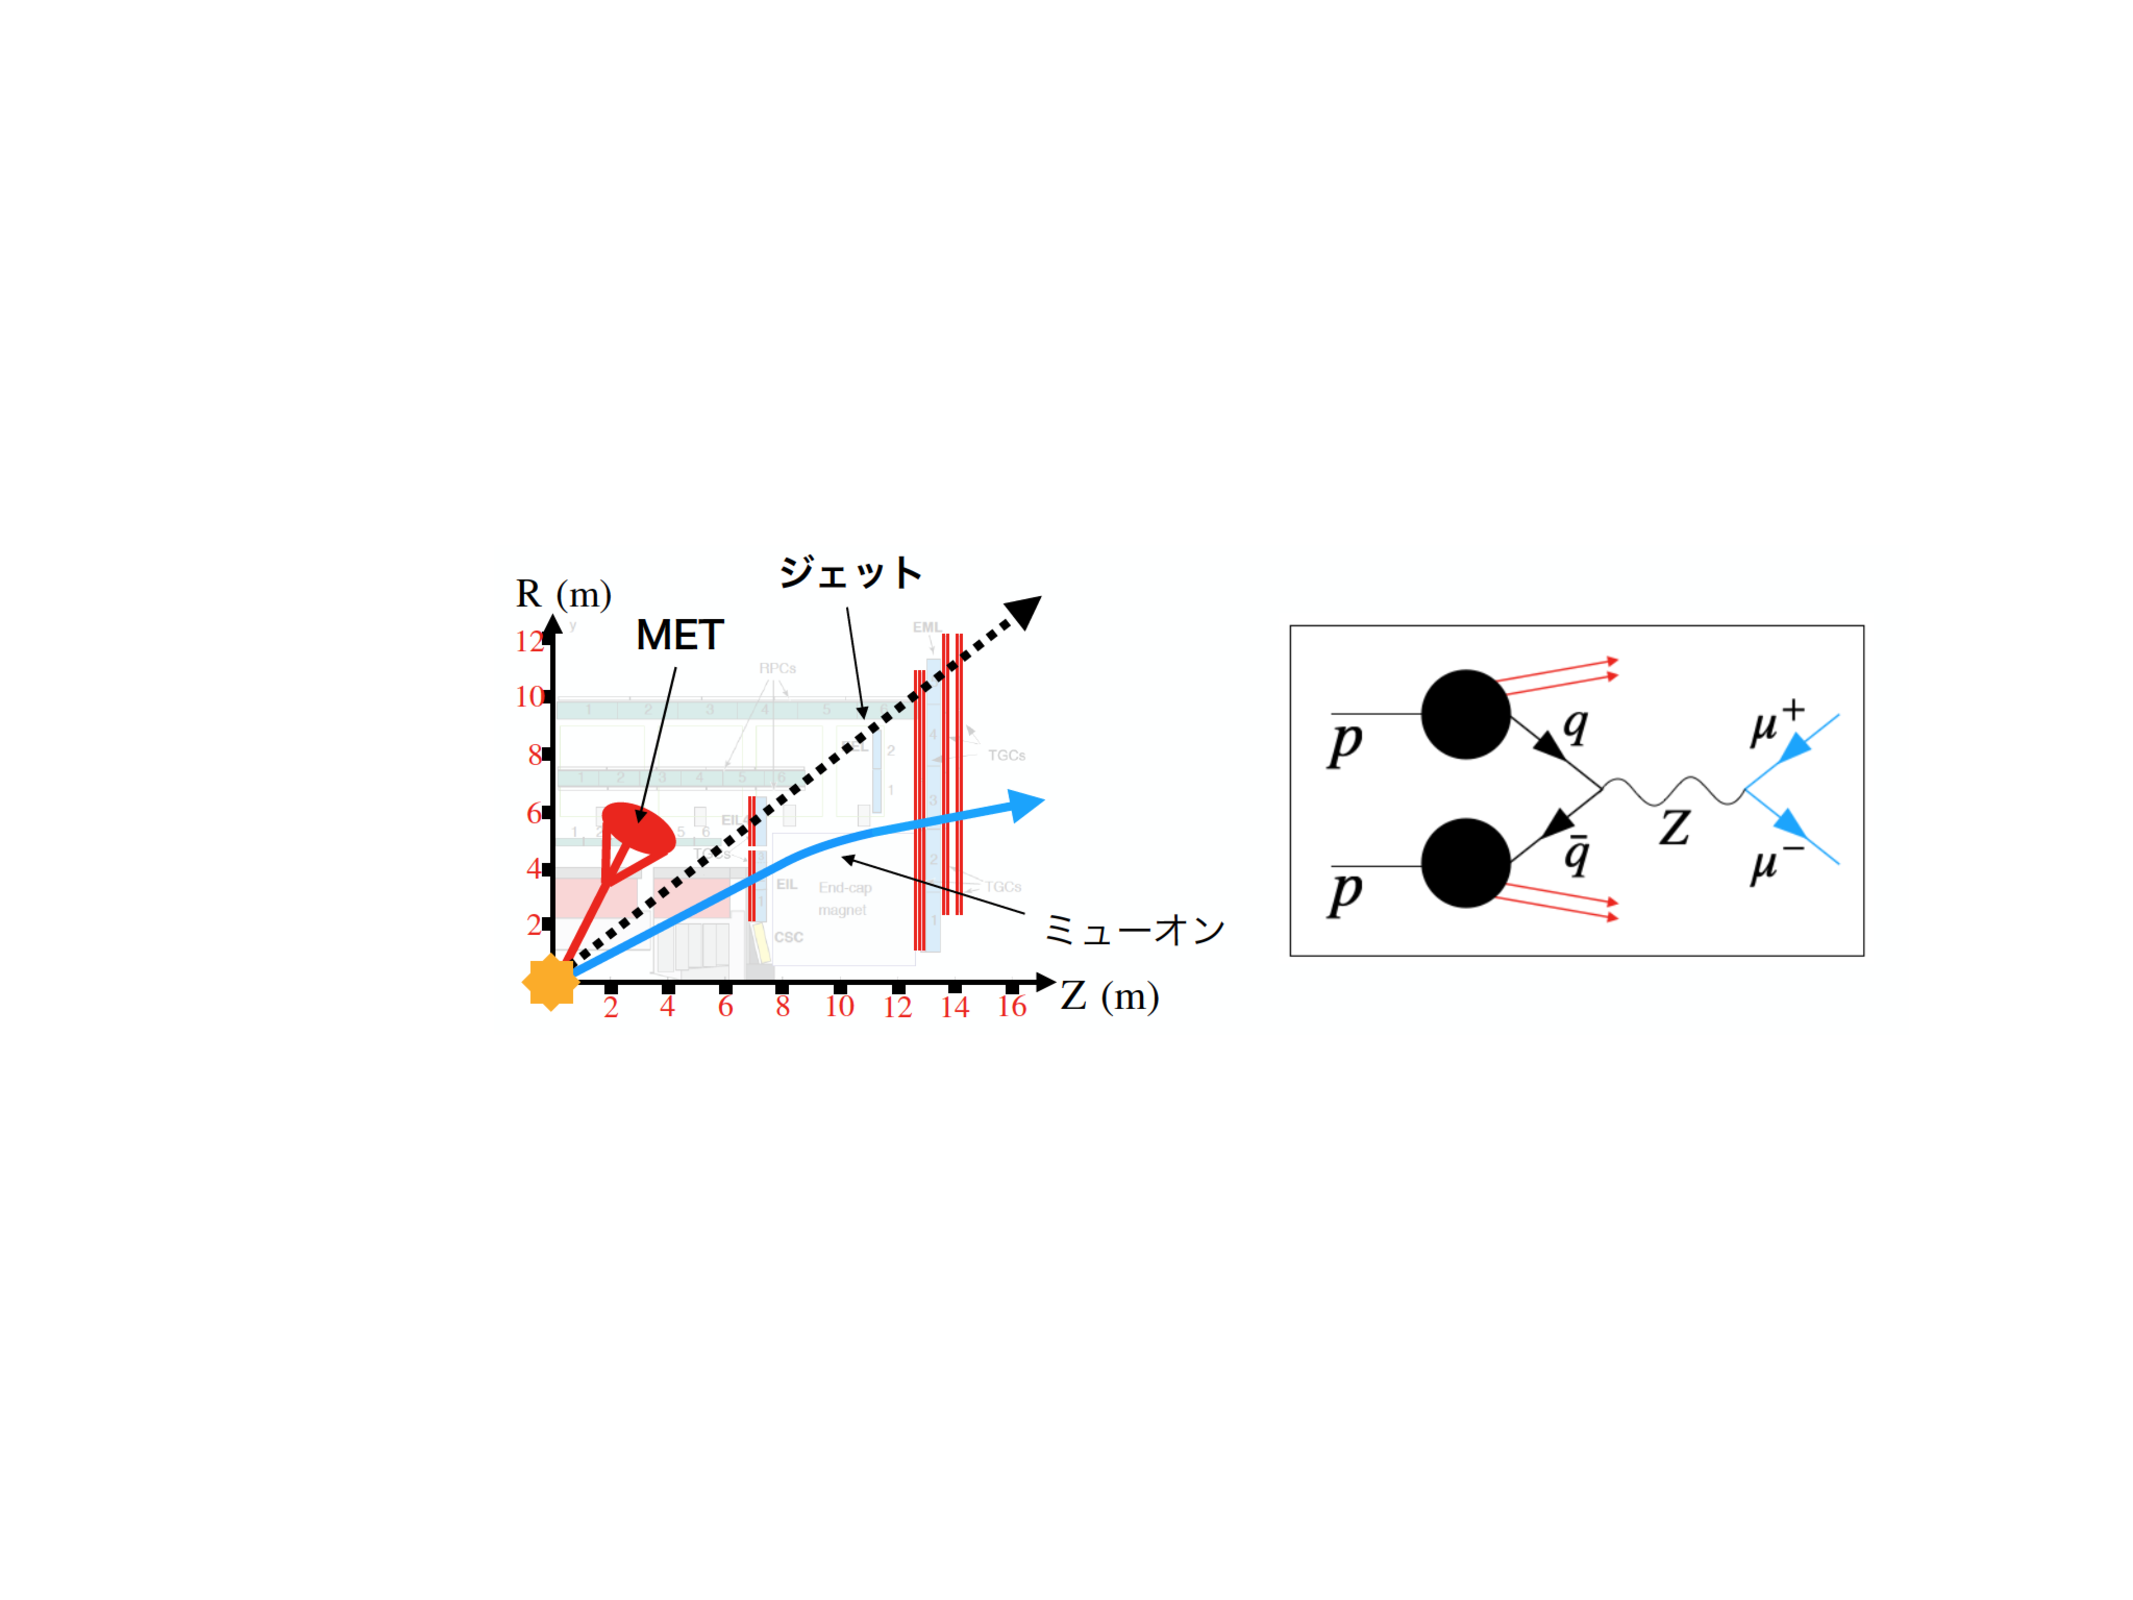
\includegraphics[width=\textwidth,page=1]{img/pdf3/met.pdf}
        \caption[遅い荷電粒子探索用トリガーが要求する事象のイメージ図]{遅い荷電粒子探索用トリガーが要求する事象のイメージ図。左図は~ATLAS~検出器における事象の様子を示している。右図は想定される崩壊過程を示して、赤が~MET~またはジェット、青がミューオン等の荷電粒子を示す。MET~またはジェットを基準バンチに要求し、ミューオン等の荷電粒子を次バンチに要求する。}
        \label{fig:met}
\end{figure}

\begin{figure}[H]
        \centering   
        \includegraphics[width=0.7\textwidth,page=3]{img/pdf3/sumi.pdf}
        \caption[スタウ粒子の速度に依存した取得効率]{スタウ粒子の速度に依存した取得効率~\cite{MT:01}。赤色、青色、緑色はそれぞれシングルミューオントリガー、遅い荷電粒子探索用トリガー、MET トリガーを示している。}
        \label{fig:sumi3}
\end{figure}

\section{本研究の目的}
\secref{sec:single}、\secref{sec:latemu}より標準的なミューオントリガーと遅い荷電粒子探索用トリガーを組み合わせれば、$0.6{\leq}\beta{\leq}1.0$の領域に感度を持つことが分かった。
\figref{fig:sumi4}は、スタウ粒子のシングルミューオントリガーおよび遅い荷電粒子探索用トリガーの速度に依存した取得効率を示している。遅い荷電粒子探索用トリガーには~MET~の要求をしていない。
緑色で示された両者の論理和を見ると$\beta\sim0.8$の領域において効率が少し低下していることが分かる。このようなことが起こる一つの原因として、ミューオン検出器の各層でのタイミング判定にずれがあることが考えられる。ミューオン検出器のある層では基準バンチ、他の層では次バンチと判定された場合、両者のトリガーを通過してしまう可能性がある。\figref{fig:time}に示したのは、粒子速度の違いにより各チェンバーに到達する時間がどれだけ変化するかを表した図である。粒子速度が小さくなるにしたがってチェンバー間の飛来にかかる時間は大きくなる。すなわち粒子の速度が遅くなるにつれてバンチ判定による一致が取れない事象が多くなりトリガー効率の低下が懸念される。以上の影響を最小限にし、トリガー効率を向上させるためには、各チェンバーにおいて判定される粒子信号のタイミング判定をより詳細に行う必要がある。各チェンバーごとにナノ秒単位のずれをそろえることで事象選別の非効率な低下を削減することができる。
ミューオン検出器におけるタイミング判定は、効率的に粒子情報を取得する上で非常に重要な要素の一つと言える。
\begin{figure}[H]
        \centering   
        \includegraphics[width=0.7\textwidth,page=4]{img/pdf3/sumi.pdf}
        \caption[スタウ粒子の速度に依存した取得効率]{スタウ粒子の速度に依存した取得効率~\cite{MT:01}。赤色、青色、緑色はそれぞれシングルミューオントリガー、遅い荷電粒子探索用トリガー~(MET~の要求なし)、両トリガー論理和を示している。}
        \label{fig:sumi4}
\end{figure}
\begin{figure}[H]
        \centering   
        \includegraphics[width=0.4\textwidth,page=4]{img/pdf3/time.png}
        \caption[粒子速度に依存した~M1~から~M3~までにかかる粒子到来時間差の変化]{粒子速度に依存した~M1~から~M3~までにかかる粒子到来時間差の変化。$|\eta|=1.4$の場合、$\beta=1.0$で$t_{\rm M13}\simeq6.7~\rm ns$、$\beta=0.8$で$t_{\rm M13}\simeq8.4~\rm ns$、$\beta=0.6$で$t_{\rm M13}\simeq11.2~\rm ns$と計算される。}
        \label{fig:time}
\end{figure}

\newpage
本研究では、ミューオン検出器の一つである~TGC~検出器に着目し、タイミング判定における詳細な見積もりおよび検証を行う。そして~TGC~検出器のタイミング調整に伴ったトリガー効率について調査し、TGC~の性能改善を目指す。光速のミューオンおよび遅い荷電粒子に対するトリガー効率の評価を行い、Run~3~に向けた感度向上に取り組む。

解析には~Run~2~における実験データおよびモンテカルロシミュレーションを用い、両者の比較、検証を行うことで問題点並びに改良点を示唆する。
Run~3~では、より詳細な新物理探索を目指す上で~Run~2~以上に精密な処理が要求される。TGC~検出器のタイミング較正により、Run~3~に向けた~TGC~検出器の最適な実装を提案する。
